\documentclass[a4paper,11pt]{book}
\newcommand{\Origin}{/home/rahul/Desktop/cfd_fossee_book/book/cfd-openfoam}

\usepackage{color}
\usepackage{layouts}
\usepackage{cclicenses}
\usepackage{morefloats}
\usepackage{paralist}
\usepackage{chngcntr}
\usepackage{layouts}
\usepackage{fancyhdr}
\pagestyle{headings}
\usepackage{amsmath,graphicx,makeidx}
\usepackage{fancybox,url}
\usepackage{cite}
%\usepackage{appendix}
\counterwithout{footnote}{chapter}
\usepackage{subfig}
\usepackage{listings}
\usepackage{varioref} % for \vref commands
%\usepackage{hyperref}

\newcommand{\redcolor}[1]{\color{red}#1\color{black}}
\newcommand{\codclr}{10pt}
\newcommand{\scilab}{Scilab}
\newcommand{\arduino}{Arduino Uno}
\newcommand{\ie}{\emph{i.e.},}

\newcommand{\ourname}[1]{\\ [1.5mm] \noindent{\bf #1}}
% Shroff book size
%\textheight 7.75in
\textheight 7.5in
\textwidth 5.5in
\evensidemargin 0.625in
\oddsidemargin 0.625in

\newcommand{\Home}{/home/rahul/Desktop/cfd_fossee_book/book/cfd-openfoam}

\newcommand{\tnfig}{0.3\linewidth}
\newcommand{\smfig}{0.45\linewidth}%0.42
\newcommand{\smfigp}{0.49\linewidth}%0.42
\newcommand{\lgfig}{0.65\linewidth}%0.65
\newcommand{\hgfig}{0.9\linewidth}

\renewcommand\bibname{References}

\newcommand{\figref}[1]{Fig.~\ref{#1}}
\newcommand{\figrefp}[1]{Fig.~\vref{#1}}
\newcommand{\tabref}[1]{Table~\ref{#1}}
\newcommand{\tabrefp}[1]{Table~\vref{#1}}
\newcommand{\chapref}[1]{Chapter~\ref{#1}}
\newcommand{\secref}[1]{Sec.~\ref{#1}}
\newcommand{\sciref}[1]{Scilab~Code~\ref{#1}}
\newcommand{\ardref}[1]{Arduino~Code~\ref{#1}}
\newcommand{\mypageref}[1]{Page~\pageref{#1}}
\newcommand{\fnref}[1]{Footnote~\ref{#1}}
\renewcommand{\topfraction}{1}
\renewcommand{\bottomfraction}{1}
\renewcommand{\textfraction}{0}
\renewcommand{\floatpagefraction}{1}
% \bibliographystyle{./IEEEtran}
\bibliographystyle{unsrt}

\hyphenation{Ashu-tosh pr-ess}

\makeindex
\begin{document}
\pagestyle{plain}
\pagestyle{empty}
\frontmatter
\thispagestyle{empty}
%\input{suppl/dedicate}
\pagestyle{headings}
\tableofcontents
\listoffigures
\listoftables
%\listofard
%\listofcode
%\thispagestyle{empty}
\addtocontents{toc}{\protect\thispagestyle{empty}}
%\input{suppl/preface}
%\input{suppl/acr}

\mainmatter
\pagestyle{headings}
\renewcommand\chaptermark[1]{\markboth{\bf {\thechapter. #1}}{}}
\renewcommand\sectionmark[1]{\markright{\bf {\thesection. #1}}}

%\input{texfiles/microcontintro.tex}
%\input{texfiles/sciaurint.tex}
%\input{suppl/intro.tex}
\chapter{Installing OpenFOAM and Paraview}
\thispagestyle{empty}
\label{sec:chap1}
\newcommand{\LocCHonefig}{\Origin/CHAPTERS/chap1/figures}

The First chapter deals with Installing OpenFOAM and Paraview. We are using Linux Operating System for installation and OpenFOAM-2.2.1 and Paraview-3.12.0.
First we will look how to install OpenFOAM and paraview using Synaptic Package Manager. Then using the downlading it from the OpenFOAM website and lastly installing
it using the source code. We will end this chapter with an example which shows running a simple problem in Paraview. As a basic requirement the user expected to have 
some basic knowledge of Computational Fluid Dynamics ( CFD ) and should be able to use basic Linux Commands.

\section{Installation using Synaptic Package Manager}

OpenFOAM and Paraview can be installed using Synaptic Package Manager. On the left side of your computer screen you can see the Launcher with the list of softwares.
Click on the search box ,Fig.\ref{search} on top of the Launcher and type Synaptic. This will display the Synaptic Package Manager. Click on it to open.

\begin{figure}[h]  
\begin{center}  
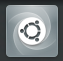
\includegraphics[scale=0.75]{\LocCHonefig/dash.png}
\caption{Search Icon on top of Launcher}
\label{search}
\end{center}  
\end{figure}

\flushleft You will be interrupted to enter the system password.

\begin{figure}[h]  
\begin{center}  
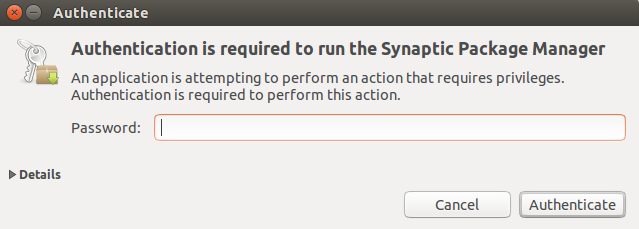
\includegraphics[scale=0.45]{\LocCHonefig/password.png}
\caption{Enter system password to open Synaptic Package Manager}
\end{center}  
\end{figure}
\vspace{1cm}

\flushleft Once the Synaptic Package Manager is Opened, in the search box type OpenFOAM.

\begin{figure}[ht]  
\begin{center}  
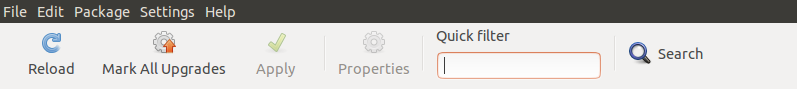
\includegraphics[scale=0.4]{\LocCHonefig/searchbox.png}
\caption{Search Box}
\label{searchbox}
\end{center}  
\end{figure}

\flushleft You will see both OpenFOAM-2.3.0 and Paraview-4.1.0. Right Click Both of them for installation and click Apply to install, Fig \ref{searchbox}. 
This might take some time to install depending upon your internet speed.

\begin{figure}[ht]  
\begin{center}  
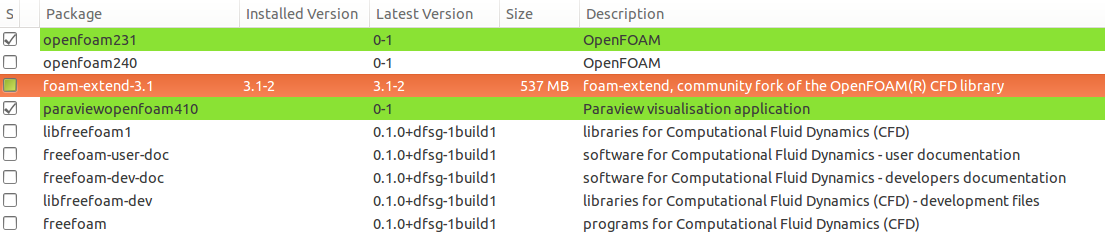
\includegraphics[scale=0.35]{\LocCHonefig/mark.png}
\caption{Install OpenFOAM and Paraview}
\label{searchbox}
\end{center}  
\end{figure}

\section{Installtion from OpenFOAM website}

\flushleft OpenFOAM can also be downloaded and installed using the OpenFOAM website. Follow the steps given below for installation. 
\begin{itemize}
\item On your browser type \textbf{www.openfoam.com/download} 
\item Go to Ubuntu Debian Installation
\item Under the first point of Installation copy the command line and paste this in your terminal window
\item Open the terminal window by pressing \textbf{Ctl+Alt+t} keys simultaneously on your keyboard or you can also open it using the 
search icon on top of the Launchbar

\begin{figure}[ht]  
\begin{center}  
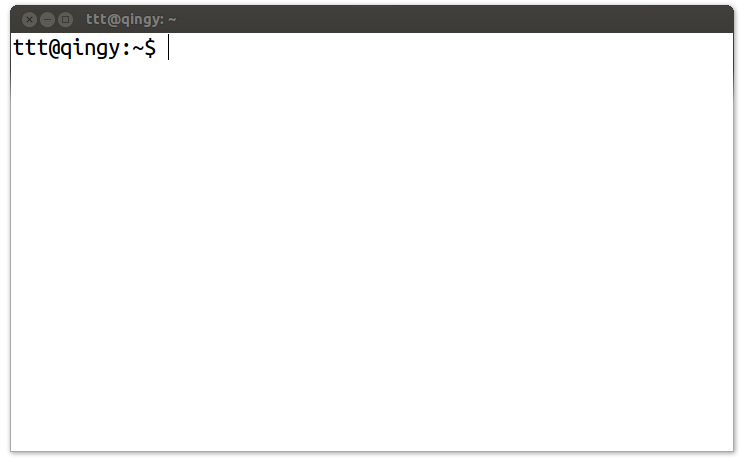
\includegraphics[scale=0.28]{\LocCHonefig/terminal.png}
\caption{Terminal window}
\label{terminal}
\end{center}  
\end{figure}

\item For complete installation for OpenFOAM and Paraview follow the steps under Ubuntu installation page

\end{itemize}

\flushleft To configure the installed software we need to edit the bashrc file. 
To do this open a new command terminal and type 
\begin{equation*}
\textbf{gedit $\sim$$\slash$.bashrc} 
\end{equation*}
and press $<enter>$

\flushleft After the bashrc file is opened scroll down to the bottom of the file. Then go back to your browser (OpenFOAM download page) and scroll down to \textbf{User Configuration}.  
Copy the line in point number 2  
\begin{equation*}
\textbf{source /opt/openfoam230/etc/bashrc} 
\end{equation*}
and paste it at the bottom of the bashrc file. Save it and close the file.

\flushleft To check if OpenFOAM is installed properly open a new command terminal and type 
\begin{equation*}
\textbf{icoFoam -help} 
\end{equation*}
and press enter. You will see a "Usage" message on your terminal screen, Fig \ref{usage} which shows that the installation is done.

\begin{figure}[ht]  
\begin{center}  
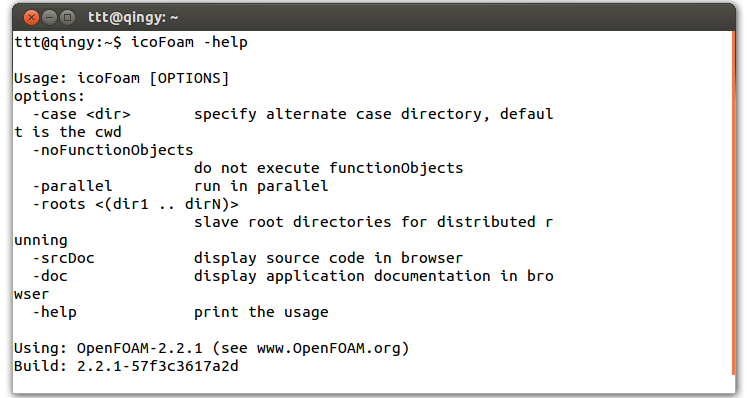
\includegraphics[scale=0.5]{\LocCHonefig/usage.png}
\caption{Usage Message}
\label{usage}
\end{center}  
\end{figure}

\flushleft Now we will set up the working directory and copy the tutorial folder. Follow the steps given below. 
\begin{enumerate}
\item Open up a new terminal and type \textbf{mkdir -p $\$$FOAM$\_$RUN} and press $<enter>$
\item Now type \textbf{cp -r $\$$FOAM$\_$TUTORIALS} \textbf{$\$$FOAM$\textunderscore$RUN} and press $<enter>$. This will copy the tutorials folder into the run directory.
\end{enumerate}

\flushleft Installation of OpenFOAM using the Debian package is now complete. Similarly you can download it for other linux OS such as Fredora, OpenSUSE.

\section{Installation using Source Code}
Alternate way to install OpenFOAM and Paraview is by Compiling the Source code available under the header of \textbf{Source Pack} Installation on the OpenFOAM website. 
Download the tar files available in \textbf{OpenFOAM.tar.gz} and \textbf{ThirdParty.tar.gz} format. Create a folder in your Home directory by the name OpenFOAM and paste the tar files in that folder and Extract the files in that folder.
Follow the steps given on the OpenFOAM source pack installation page to complete the installation. Since we compile the source code it might take a few hours to complete.

\section{Example Problem - Lid Driven Cavity}
We will solve an problem here by the name Lid Driven Cavity. It is a two dimensional problem where the upper plate moves and other three sides of the plate are fixed / stationary, \ref{lid}. 
The solver we use here is icoFoam which is an Transient solver for incompressible flow.

\begin{figure}[ht]  
\begin{center}  
\includegraphics[scale=0.3]{\LocCHonefig/geometry1.png}
\caption{Lid Driven Cavity}
\label{lid}
\end{center}  
\end{figure}

In the terminal type the path given below :\newline

\small{cd OpenFOAM/OpenFOAM-2.3.0/run/tutorials/incompressible/icoFoam/cavity} \newline

\subsection*{Meshing the geometry}
We need to mesh the geometry. This can be done using the blockMesh utility of OpenFOAM. In the command terminal type \textbf{blockMesh} and press $<enter>$ which completes the meshing, Fig \ref{mesh}

\begin{figure}[ht]  
\begin{center}  
\includegraphics[scale=0.3]{\LocCHonefig/blockMesh.png}
\caption{blockMesh for meshing}
\label{mesh}
\end{center}  
\end{figure}

\newpage

\subsection*{Solving}
Once meshing is done we now run the solver by typing : \\
\center \textbf{icoFoam} \\
\flushleft in the command terminal and press $<enter>$. The iteration running can be seen in the terminal window,Fig \ref{solver}. \newline
\flushleft We have now solved the lid driven cavity case.

\begin{figure}[ht]  
\begin{center}  
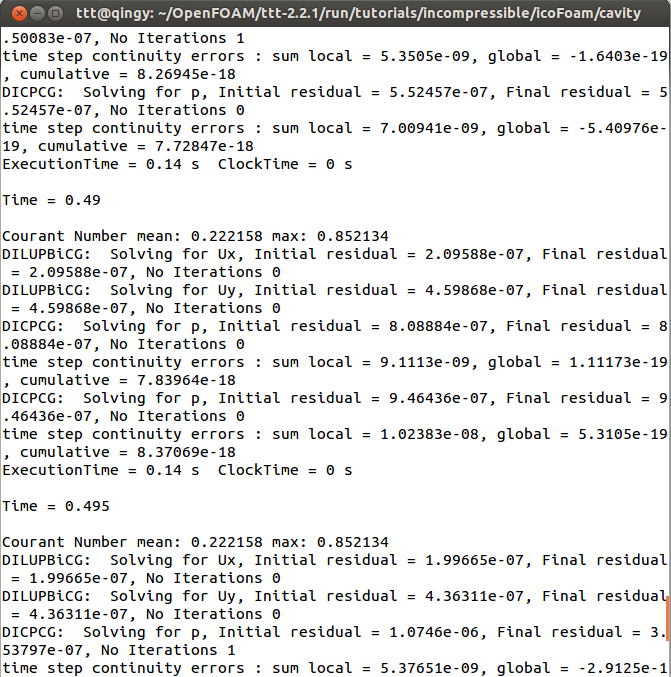
\includegraphics[scale=0.3]{\LocCHonefig/solver.png}
\caption{Iteration on Terminal Window}
\label{solver}
\end{center}  
\end{figure}

\subsection*{Visualization}
To Visualize the results we use Paraview. To open paraview in your terminal type \\
\center \textbf{paraFoam} \\
\flushleft and press $<enter>$. This will open up the paraview window, Fig \ref{pv}.

\begin{figure}[ht]  
\begin{center}  
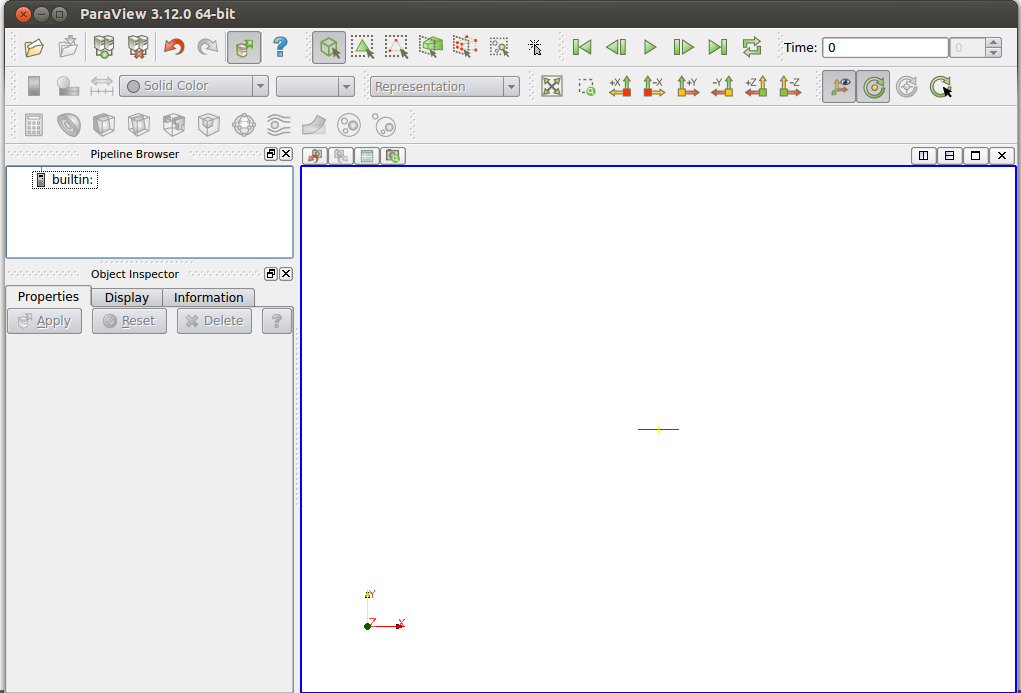
\includegraphics[scale=0.32]{\LocCHonefig/paraview.png}
\caption{Paraview window}
\label{pv}
\end{center}  
\end{figure}

\flushleft Click on the Apply button on the left hand side of the \textbf{Object Inspector} Menu to view the Geometry, Fig\ref{geom}.

\begin{figure}[ht]  
\begin{center}  
\includegraphics[scale=0.32]{\LocCHonefig/geometry.png}
\caption{Geometry}
\label{geom}
\end{center}  
\end{figure}

\flushleft This brings us to the end of the first chapter. To summaries we have learnt to Install OpenFOAM and Paraview and ran a test example. 
The next chapter will cover about creating simple geometry in OpenFOAM.
 %rahul  
\chapter{Creating a Simple Geomtery in OpenFoam}
\thispagestyle{empty}
\label{sec:chap2}
\newcommand{\LocCHtwofig}{\Origin/CHAPTERS/chap2/figures}

In this chapter we will learn how to create a simple geometry in OpenFOAM using the blockMeshDict utility of OpenFOAM. We can create simple geometries
like a square, rectangle , circular cylinder using blockMeshDict.

\section{Geometry creation}
Here we will use the lid-driven cavity problem example mentioned in the previous chapter for the pre-processing. As previously mentioned you can type the following path in the command terminal to open the id-driven cavity problem:
\small{cd OpenFOAM/OpenFOAM-2.3.0/run/tutorials/incompressible/icoFoam/cavity}\newline
\flushleft After this if you type “ls” in the command terminal would see three folder inside it given as:

\begin{itemize}
\item 0
\item constant
\item system
\end{itemize}

\flushleft where the 0 folder gives the initial boundary conditions, constant gives the geomtery file and system folder gives the number of the iterations the solver would run along other important files. You can find the boundary of the problem in a polymesh folder inside constant. In order to open that type the following in the command terminal and then press $<enter>$:
\center \textbf{cd constant/polymesh}
\flushleft Then type ls to in the command terminal and press $<enter>$. This shows the geomtery file given as blockMeshDict file. In order to view this file type the following in the command terminal:

\center \textbf{gedit blockMeshDict}

\flushleft where gedit it the name of the editor we have used. Note that you may use any other text file editor to view and edit this file.
\flushleft Now you can see the gedit window containing the geometry file. In order to draw a geomtery in OpenFoam you need to follow the below mentioned instructions.
\flushleft In openFoam a geomtery is broken down into small blocks and are then numbered starting from 0, as shown in the Fig \ref{geometry}

\begin{figure}[ht]  
\begin{center}  
\includegraphics[scale=0.32]{\LocCHtwofig/geometry1.png}
\caption{geomtery points of the lid driven cavity}
\label{geometry}
\end{center}  
\end{figure}
 
\section{blockMeshDict} 
\flushleft Note that in openFoam to create a 2-D geometry you need to give a unit cell thickness in the Z axis. Now in order to create a new geomtry file open a new folder in destop and rename it a “blockMeshDict”. 
\flushleft A blockMeshDict file basically has the following parts:

\begin{itemize}
\item Foam File details
\item vertices
\item blocks
\item edges
\item boundary
\item mergepatchpairs
\end{itemize}

\flushleft Note that the line convertToMeter gives unit in which the geomtery is drawn. For example, as we are drawing the geomtery in meters for this problem we will keep convertToMeters as 1. Now after opening the new blockMeshDict file created in the desktop copy the lines from initial Foam File till convertToMeters from the old file and paste it. After this type vertices and then you can give the X, Y and Z co-ordinates of the boundary as shown below:

\begin{figure}[ht]  
\begin{center}  
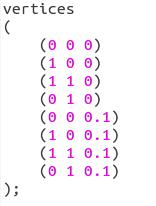
\includegraphics[scale=0.66]{\LocCHtwofig/vertices.png}
\caption{coordinates of boundary geomtery points of the lid driven cavity}
\label{vertices}
\end{center}  
\end{figure}

\flushleft Then type block, inside which you give the details of the boundary co-ordinates along with the number of mesh divisions in X, Y and Z direction in the following way, fig \ref{blocks}:

\begin{figure}[ht]  
\begin{center}  
\includegraphics[scale=0.66]{\LocCHtwofig/blocks.png}
\caption{block details of the geomtery}
\label{blocks}
\end{center}  
\end{figure}

\flushleft Here hex represents hexahedral block and the number next to that gives the names of the points at the boundary in clock-wise direction to form a block. Note that for more than one blocks the number of points would be more. The number of grid points can be modified as per requirement. For this problem we have used a 2-D mesh having 30x30 divisions and unit dept. Now since we have all straight edges in this geometry, we will keep the egdes empty.

\begin{figure}[ht]  
\begin{center}  
\includegraphics[scale=0.66]{\LocCHtwofig/edges.png}
\caption{edge details of the geomtery}
\label{edges}
\end{center}  
\end{figure}
\vspace{2cm}
\flushleft Next we give the details of the boundary. In the geometry we can see the following boundary conditions,as shown in fig \ref{boundary}:
\begin{itemize}
  \item moving wall
  \item fixed wall
  \item front and back
\end{itemize}
\begin{figure}[ht]  
\begin{center}  
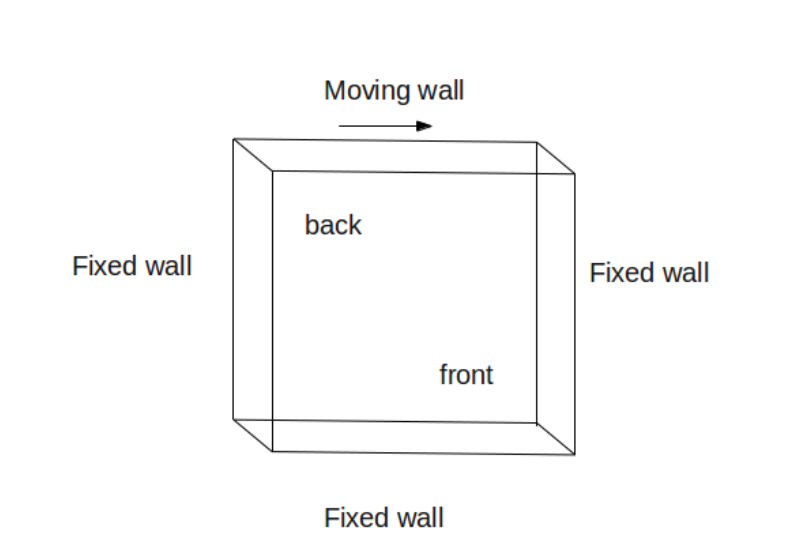
\includegraphics[scale=0.45]{\LocCHtwofig/boundary.png}
\caption{boundary names of the geomtery}
\label{boundary}
\end{center}  
\end{figure}
\flushleft where it has a top moving wall and three fixed wall. The front and back faces are kept empty as this is a 2-D problem. 
\vspace{10cm}
\flushleft Now in the blockMeshDict file you can type the boundary as shown in fig \ref{boundary_name}:
\begin{figure}[ht]  
\begin{center}  
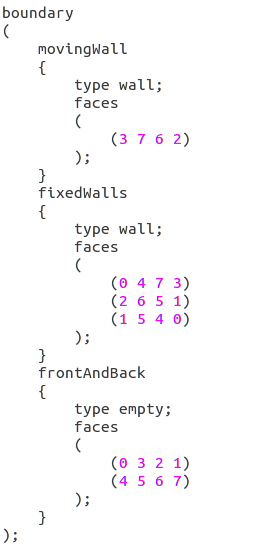
\includegraphics[scale=0.66]{\LocCHtwofig/boundary_name.png}
\caption{boundary details of the geomtery}
\label{boundary_name}
\end{center}  
\end{figure}


\flushleft Here within the boundary names enter the type of boundary used and  then faces, giving the points of the block forming a particular boundary. Note that you should be very careful while writing the order of the points. The order should be such that if you place a folded palm on the surface of a boundary the thumb should be pointing normal to the surface and the fingers should be folded such that they make a curl in clockwise or anti-clockwise direction. Note that you should use either clockwise or anti-clockwise convention throughout the file and but not both. Also you should be very careful regarding openning and closing of brackets in this file.

\flushleft After this$,$ in a new line type mergePatchPairs. Since in this problem we do not have to merge any patches we will keep this empty$,$ fig \ref{merge}.
\vspace{0.32cm}
\begin{figure}[ht]  
\begin{center}  
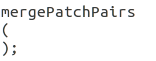
\includegraphics[scale=0.66]{\LocCHtwofig/merge.png}
\caption{merge patch details of the geomtery}
\label{merge}
\end{center}  
\end{figure}

\flushleft Note that two “P”'s are capital here.
\flushleft After completing writing this file save it and close this file. Thus you have learned ho wto create a geomtery file.
\flushleft Now go back to the command terminal and type the following twice to go back to cavity folder:

\center \textbf{cd ..} 

\flushleft Next you can mesh this geomtry by typing blockMesh in the command terminal. After this you can view the geometry by opening paraview. For this type paraFoam in the command terminal and press $<enter>$.
\flushleft In the paraview window press Apply button on the left hand side of the Object Inspector Menu to
view the Geometry, as shown in the fig \ref{paraview1}:
\begin{figure}[ht]  
\begin{center}  
\includegraphics[scale=0.32]{\LocCHtwofig/paraview1.png}
\caption{Paraview window showing the 2-D geometry}
\label{paraview1}
\end{center}  
\end{figure}

\flushleft As you as learned in the previous chapter, you can use different feature in the paraview window to check the details of the geometry.
 %suba
\chapter{Creating a Curved Geomtery in OpenFoam}
\thispagestyle{empty}
\label{sec:chap3}
\newcommand{\LocCHthreefig}{\Origin/CHAPTERS/chap3/figures}


In this chapter we will learn how to create a 2-D geometry for a flow over a cylinder. As it is an axis-symmetric geometry, we will consider the cylinder as a semi-circle and a rectangular domain around it. For meshing this geometry you should divide the domain into small hexahedral blocks. In this particular problem we have body fitted grid, as shown in Fig \ref{frontface} and Fig \ref{backface}{$:$}

\begin{figure}[ht]  
\begin{center}  
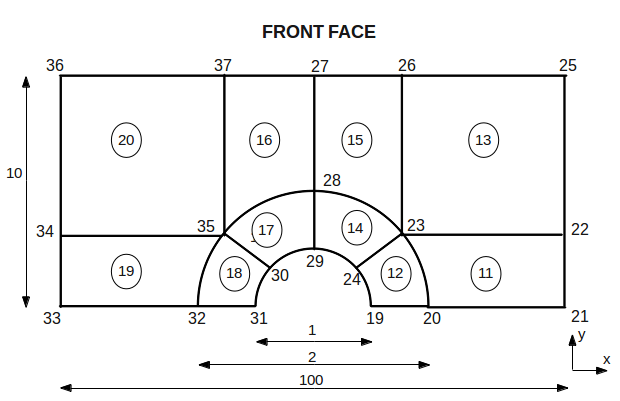
\includegraphics[scale=0.6]{\LocCHthreefig/frontface.png}
\caption{Geomtery points in the front face for 2-D flow over a cylinder}
\label{frontface}
\end{center}  
\end{figure}

\begin{figure}[ht]  
\begin{center}  
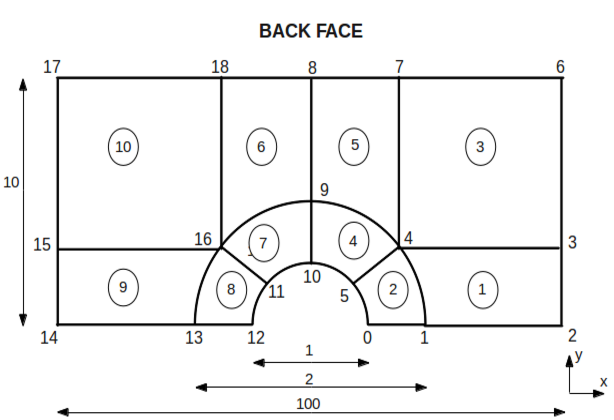
\includegraphics[scale=0.6]{\LocCHthreefig/backface.png}
\caption{Geomtery points in the back face for 2-D flow over a cylinder}
\label{backface}
\end{center}  
\end{figure}

\flushleft Now, as mentioned in the previous chapter create a new blockMeshDict file and open it. In this geometry file  copy the initial few lines  till “convertToMeters” from previous lid-driven cavity problem “blockMeshDict” file and paste it. Here we will keep “convertToMeters” as 1 as we have given the geometry in meters. After this write down the coordinates of the vertices of the geometry in a similar fashion as given in the previous chapter. 
\flushleft For this particular problem we have used cosine and sine function to calculate the vertices on the curved edges as shown below{$:$}

\begin{figure}[ht]  
\begin{center}  
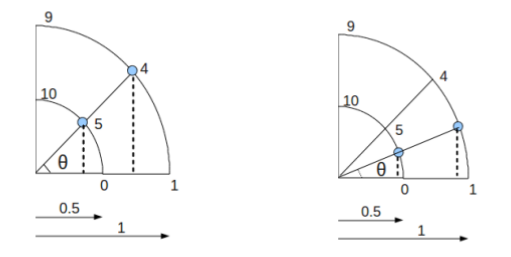
\includegraphics[scale=0.6]{\LocCHthreefig/angle.png}
\caption{Geomtery points for 2-D flow over a curved body}
\label{angle}
\end{center}  
\end{figure}

\flushleft where angle {$\theta$}  is calculated as{$:$}
\flushleft sin({$\theta$}) = perpendicular/hypotenuse
\flushleft cos({$\theta$}) = base/hypotenuse
\flushleft Note that you should be very careful about the order of the vertex coordinates. It should start from 0 and be continued as 1,2,3.., as shown below{$:$}
\flushleft vertices
\flushleft(
\flushleft  (0.5 0 0)	//0
\flushleft  (1 0 0)	//1
\flushleft.
\flushleft.
\flushleft.
\flushleft.
\flushleft);
\flushleft After this enter the details within blocks in a similar manner as shown in the previous chapter. Here in this problem, we have divided the geometry domain into ten small hexahedral blocks having structured body fitted grid points, as shown in fig \ref{blocks}. For further details on how to create blocks you may refer to chapter 2.

\begin{figure}[ht]  
\begin{center}  
\includegraphics[scale=0.6]{\LocCHthreefig/blocks.png}
\caption{Block details for the blockMeshDict file}
\label{blocks}
\end{center}  
\end{figure}

\flushleft In the previous chapter we have seen, the geometry domain had staright edges, thereby we had kept the details within edges keyword  empty (which is the default condition). But here, in this geometry we have curved edges. In OpenFOAM we can use the following types of edges in blockMeshDict file, as shown in fig \ref{ref}{$:$}

\begin{figure}[ht]  
\begin{center}  
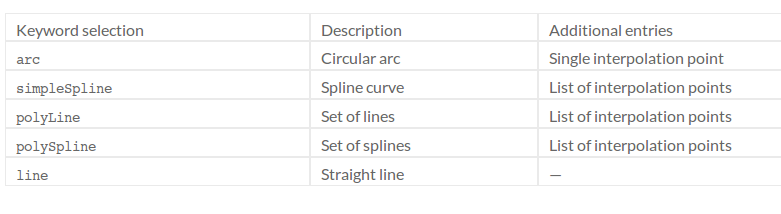
\includegraphics[scale=0.6]{\LocCHthreefig/ref.png}
\caption{Types of edges used in BlockMeshDict dictionary}
\label{ref}
\end{center}  
\end{figure}

\flushleft For this problem we have used arc edges. Therfore the details within edges can be given as{$:$}
\flushleft edges
\flushleft (
 \flushleft{$<$}keyword{$>$} {$<$}vertices joining the edge{$>$} (interpolation points)
\flushleft);
\flushleft The details of edges for our current problem is given in fig \ref{edges}{$:$}

\begin{figure}[ht]  
\begin{center}  
\includegraphics[scale=0.7]{\LocCHthreefig/edges.png}
\caption{Edge details for the blockMeshDict file}
\label{edges}
\end{center}  
\end{figure}

\flushleft After this enter the boundary patches under the keyword boundary. You may refer to the previous chapter to get know more details regarding how to write the boundary patches.
\flushleft Similar to the lid-driven cavity problem , even this geometry does not have any patches to be merged. Therefore we will keep the mergePatchPairs empty.
\flushleft After completing the blockMeshDict file, you can save it within the required case file in polymesh folder inside constant folder. Thereafter switch back to the command terminal and open the required case file as mentioned in the previous chapter.
\flushleft After this enter blockMesh in the command terminal and press $<enter>$. Thus you can see geometry is meshed. After this type paraFoam in the command terminal and press{$<$}enter{$>$}. This opens the ParaView window. Now on the ParaView window press apply on the left hand side of the Object Inspector Menu to view the new geometry.

\begin{figure}[ht]  
\begin{center}  
\includegraphics[scale=0.25]{\LocCHthreefig/paraview1.png}
\caption{ParaView window showing the 2-D geometry}
\label{paraview1}
\end{center}  
\end{figure}

\flushleft Now in the ParaView window you can check or uncheck the different regions within the mesh region in  the Object Inspector Menu to visualize differnt regions on the geomtery. You can also visualize the geometry in wire-frame instead of surface by changing it from the down-down Active Variable Control Menu.
\flushleft Thus in this chapter we learned how to create a curved geometry in OpenFOAM and visualize it in different ways using ParaView.
 %suba
\chapter{Simulating flow in a Lid Driven Cavity using OpenFOAM}
\thispagestyle{empty}
\label{sec:chap4}
\newcommand{\LocCHfourfig}{\Origin/CHAPTERS/chap4/figures}


In this chapter we would learn how to solve a lid driven cavity problem using icoFoam solver and viewing the results in ParaView. As you might recollect from the 2nd chapter we, learned how to create the case file in OpenFoam and write its blockMeshDict file.
You may review the previous chapter to see the problem statement for a lid driven cavity. Here in this problem we have a rectangular box of unit thickness with top surface moving with a velocity of 1 m/s and the other three sides fixed, as shown in fig \ref{geometry}$:$ 
Here we have considered a Re of 100.

\begin{figure}[ht]  
\begin{center}  
\includegraphics[scale=0.4]{\LocCHfourfig/geometry.png}
\caption{Geomtery of 2-D lid driven cavity}
\label{geometry}
\end{center}  
\end{figure}

\flushleft Now to solve our present problem open acommand terminal by pressing $<$ctrl$>$, $<$Alt$>$ and $<$T$>$ simulataneously. After this enter the path for the current case file as shown below$:$
\flushleft cd run/tutorial/incompressible/icoFoam/cavity
\flushleft After openning the required case file enter 'ls'. This would show the folders within this case file. Here as mentioned in chapter 2 you would find three folders by the name$:$

\begin{itemize}
  \item 0
  \item constant
  \item system
\end{itemize}

\flushleft Now if you press 'cd 0' <enter> and then 'ls' <enter> in the command terminal, you would find two folders given as$:$

\begin{itemize}
  \item P
  \item U
\end{itemize}

\flushleft These folders gives the initial boundary conditions for pressure (i.e. P), velocity (i.e. U), temperature, etc of the geomtery. After this go back to the cavity folder by typing 'cd ..' $<$enter$>$.
\flushleft Now if you open the constant folder by entering 'cd constant' <enter> in the command terminal followed by 'ls' <enter> you would find two folder$:$

\begin{itemize}
  \item polyMesh
  \item transportProperties
\end{itemize}

\flushleft Here polyMesh folder contains the blockMeshDict file. You can open this by typing 'cd poymesh' $<$enter$>$ followed by 'ls' $<$enter$>$ in the command terminal and then type 'gedit blockMeshDict'. This would show you the blockMeshDict file in text editor which contains the veritces, blocks and boundary patches of the geometry. The tranportProperties contain properties of the fluid medium used in this this problem. 
\flushleft Now you can go back to the cavity folder by entering cd .. twice in the command terminal. After this type 'cd system' <enter> followed by 'ls' $<$enter$>$. This would show you the three folders within system file.
\begin{itemize}
  \item ControlDict
  \item fvSchemes
  \item fvSolution
\end{itemize}

\flushleft Here controlDict file contains control parameters for start and stop of the number of iterations, fvSolution contain discretization schemes used for simualtion of this problem and fvSchemes contains equations for solver, tolerance, etc.
\flushleft To mesh the geometry go back to the cavity folder in the command terminal and enter the following and press $<$enter$>$:
\flushleft blockMesh
\flushleft This would mesh the geometry as shown in the fig \ref{blockmesh}$:$

\begin{figure}[ht]  
\begin{center}  
\includegraphics[scale=0.7]{\LocCHfourfig/blockMesh.png}
\caption{Meshing of the 2-D geometry in OpenFOAM}
\label{blockmesh}
\end{center}  
\end{figure}

\flushleft As you can see, we have used course mesh for this problem. If there are some error in the blockMesDict file, it would be shown in the command terminal. You can also type 'checkMesh' $<$enter$>$ in the command terminal to check the different properties of the meshed geometry like number of cells, skewness, etc. 
\flushleft After this to view the meshed geometry, you can type 'paraFoam' $<$enter$>$ in the command terminal. This woould open the ParaView window. Now on the ParaView window press apply on the left hand side of the Object Inspector Menu to view the meshed geometry, as shown in fig \ref{paraview1}. After inspecting the geomety you may close the ParaView window and switch back to the command terminal.

\begin{figure}[ht]  
\begin{center}  
\includegraphics[scale=0.32]{\LocCHfourfig/paraview1.png}
\caption{Visualization of the 2-D geometry in ParaView}
\label{paraview1}
\end{center}  
\end{figure}

\flushleft Now for simulating this particular problem we have used icoFoam solver. This is a Transient solver for incompressible, laminar flow of Newtonian fluids. To solve this problem type 'icoFoam' <enter> in the command terminal. You can see the progressing iterations in the terminal window along with the residual values. After it ends type 'paraFoam' $<$enter$>$ in the terminal window for post-processing. 
\flushleft This would open the ParaView window. As mentioned previously press apply on the left hand side of the Object Inspector Menu to view the new geometry. After this you can check or uncheck the different regions within the mesh region in  the Object Inspector Menu to visualize differnt regions on the geomtery. Now to check the velocity contours select U from the drop-down Active Variable Control Menu, from the visible toolbar. This will show the initial velocity countour of the cavity, as shown in fig \ref{vel1}. Along with this you may also select the Toggle Colour Legend from the toolbar to visualize the legend.

\begin{figure}[ht]  
\begin{center}  
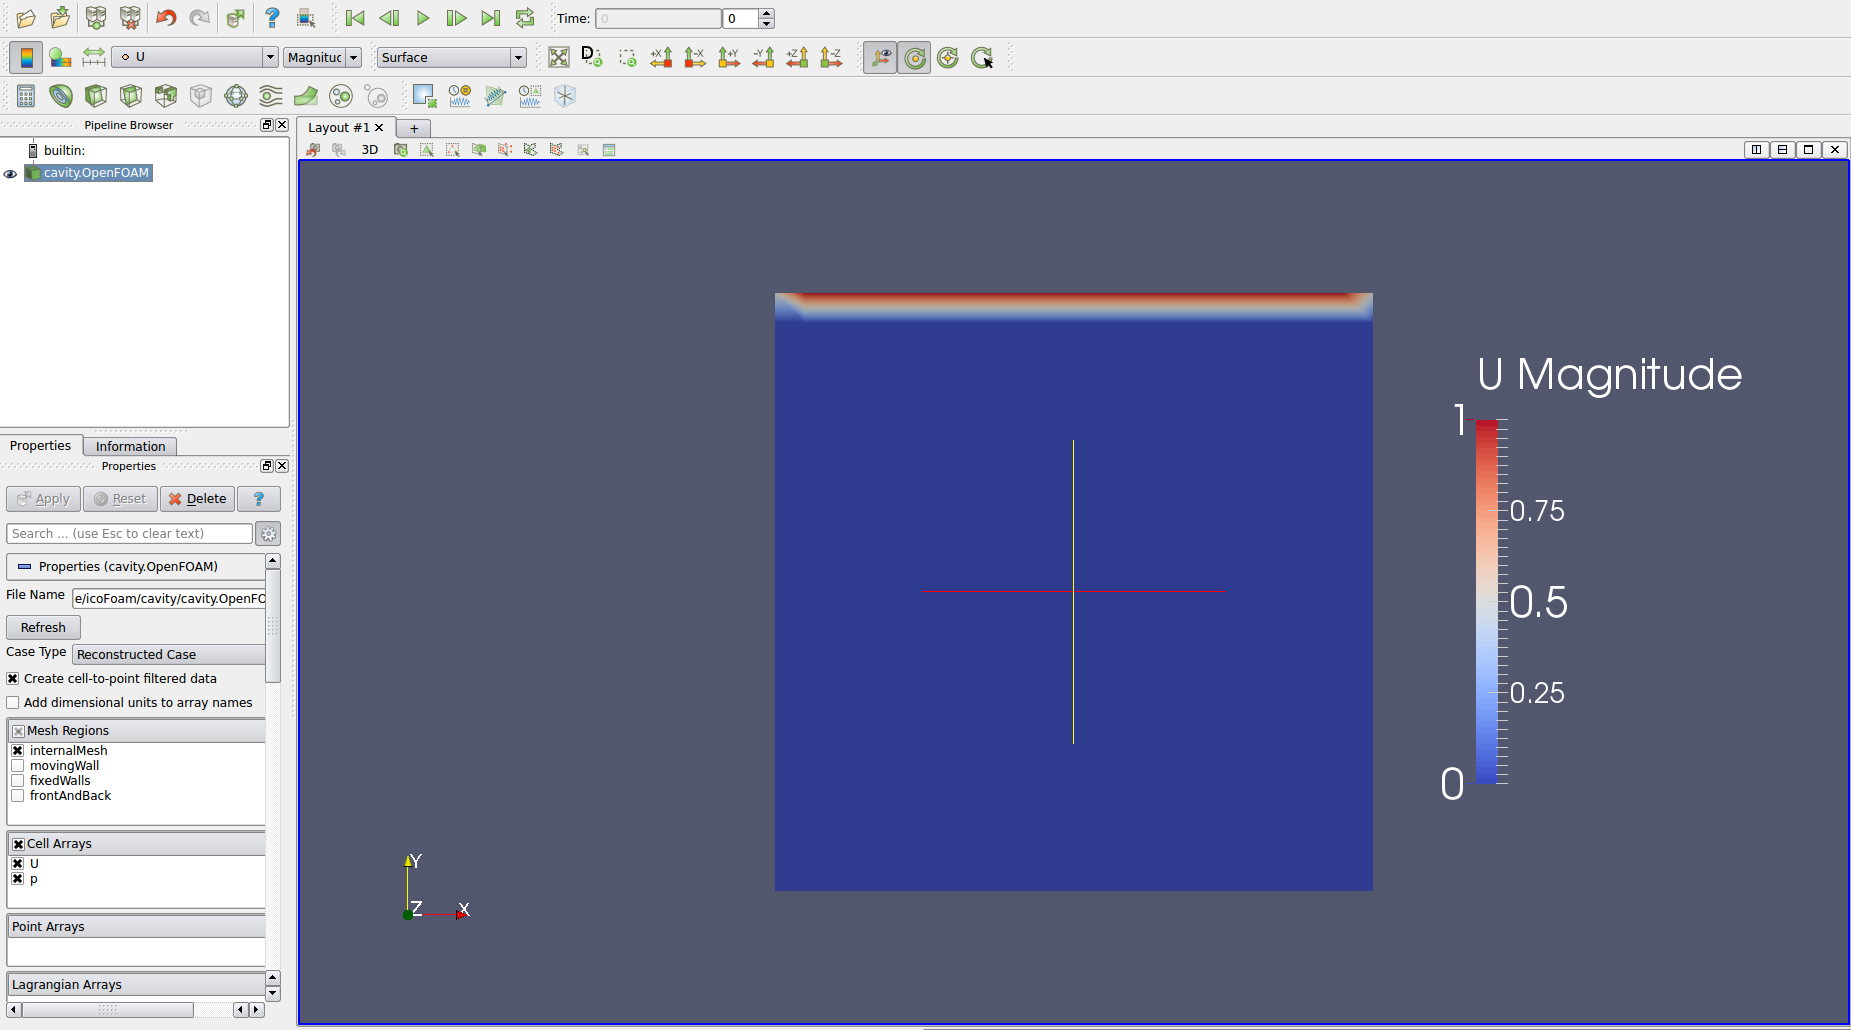
\includegraphics[scale=0.24]{\LocCHfourfig/vel1.png}
\caption{Velocity contour in the 2-D geometry at time 0 sec in ParaView}
\label{vel1}
\end{center}  
\end{figure}

\flushleft Now in the paraView window press the 'play' buttom from the VCR control. This would visualize the changing velocity countour along with the progressing iterations. You can see the final velocity contour as shown in fig \ref{vel2}.

\begin{figure}[ht]  
\begin{center}  
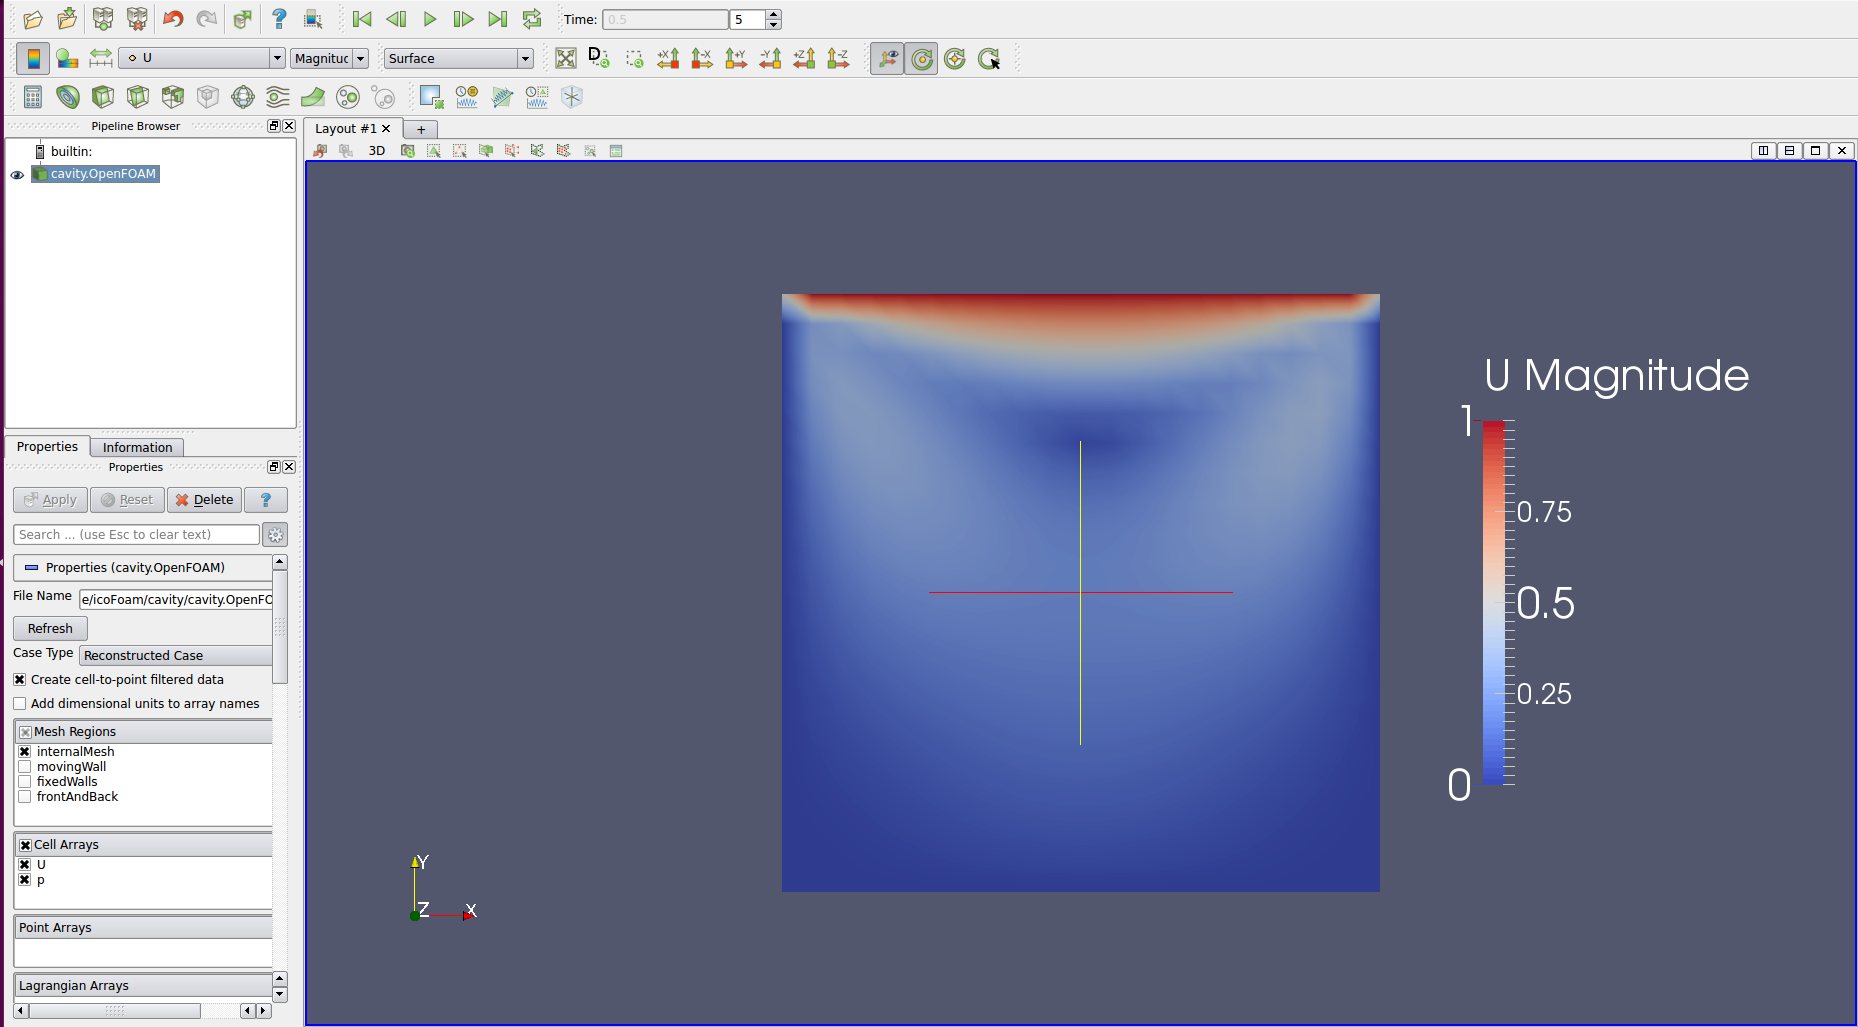
\includegraphics[scale=0.24]{\LocCHfourfig/vel2.png}
\caption{Velocity contour in the 2-D geometry at final state in ParaView}
\label{vel2}
\end{center}  
\end{figure}

\flushleft Now to validate our result we need to plot the u and v velocity in the domain. To do this click on the 'plot over line' object from the  Active Variable Control Menu bar. Now for our validation we need to plot u/U versus l/L in the X and Y axis. To do this select X-axis on the left hand side  Object Inspector Menu. This will show you the Pressure and velocity plot along X-direction.

\begin{figure}[ht]  
\begin{center}  
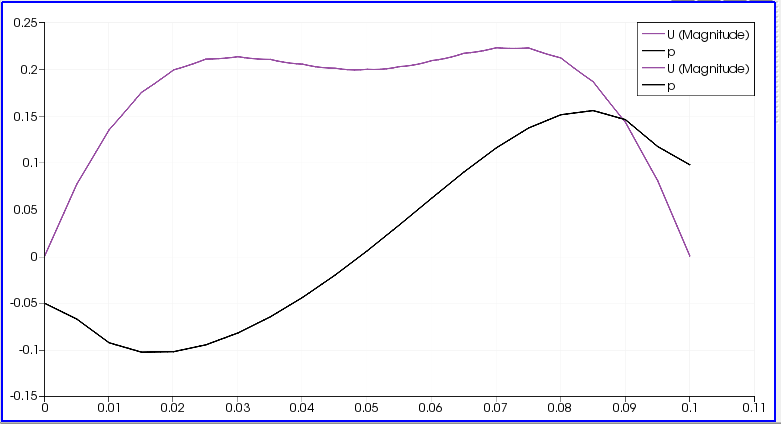
\includegraphics[scale=0.24]{\LocCHfourfig/xaxisvel.png}
\caption{Velocity contour in the 2-D geometry at final state in ParaView}
\label{xaxisvel}
\end{center}  
\end{figure}

\flushleft On selecting the Yaxis you will see the velocity along Y-axis.

\begin{figure}[ht]  
\begin{center}  
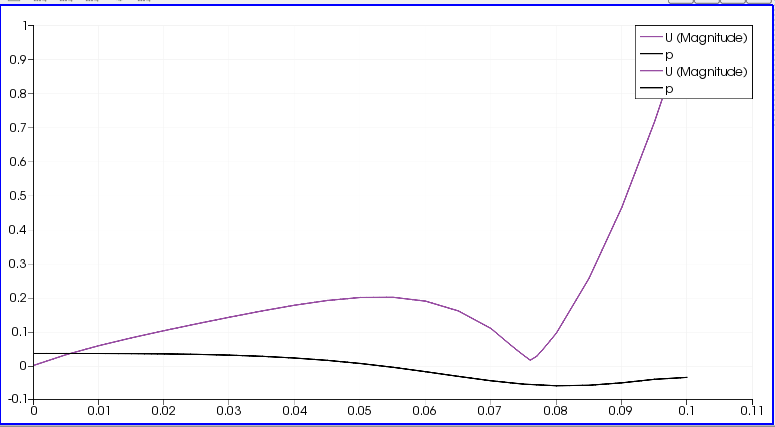
\includegraphics[scale=0.24]{\LocCHfourfig/yaxisvel.png}
\caption{Velocity contour in the 2-D geometry at final state in ParaView}
\label{yaxisvel}
\end{center}  
\end{figure}

\flushleft Now you may save these data by selecting File>Save As> and then give appropriate file name. These data will be saved in .csv format. After this open this file from home folder in libreoffice sheet. In the office sheet you can copy paste U:0 and P:1 on a new sheet and calculate it as U:0/U and P:1/L. And them plot them using chart utility. This would give you the following result.
 %suba
\chapter{Supersonic flow over a wedge using OpenFOAM}
\thispagestyle{empty}
\label{sec:chap5}
\newcommand{\LocCHfivefig}{\Origin/CHAPTERS/chap5/figures}


In this chapter we would learn how to simulate a supersonic flow over a wedge and post-process it using ParaView. Here the domain for simulation is given as shown in fig \ref{geometry}$:$

\begin{figure}[ht]  
\begin{center}  
\includegraphics[scale=0.7]{\LocCHfivefig/geometry.png}
\caption{Geomtery of 2-D wedge along with boundary conditions}
\label{geometry}
\end{center}  
\end{figure}

\flushleft Please note that this chapter in written assuming the readers have some prior know on compressible flows and gas dynamics.

\flushleft As shown in the figure, in this problem statement we have a wedge at 15 degree with the horizontal and a flow from the inlet at 5 m/s. The boundary conditions used in the geometry file are similar to that as shown in the figure. Now this test case is already pready in the tutorial directory of OpenFoam. Thereby in this chapter we would mainly focus on how to simulate compressible flow over a given test case rather than creating a geometry. 
\flushleft Now to solve our present problem open acommand terminal by pressing $<$ctrl$>$, $<$Alt$>$ and $<$T$>$ simulataneously. After this enter the path for the current case file as shown below$:$
\flushleft cd run/tutorial/compressible/rhoCentralFoam/wedge15Ma5
\flushleft After openning the required case file enter 'ls'. This would show the folders within this case file. Here as mentioned in chapter 2 you would find three folders by the name$:$

\begin{itemize}
  \item 0
  \item constant
  \item system
\end{itemize}

\flushleft Now if you press 'cd 0' <enter> and then 'ls' $<$enter$>$ in the command terminal, you would find two folders given as:

\begin{itemize}
  \item P
  \item U
  \item T
\end{itemize}

\flushleft These folders gives the initial boundary conditions for pressure (i.e. P), velocity (i.e. U), temperature (i.e. T), etc of the geomtery. After this go back to the wedge folder by typing 'cd ..' $<$enter$>$.
\flushleft Now if you open the constant folder by entering 'cd constant' $<$enter$>$ in the command terminal followed by 'ls' <enter> you would find two folder$:$

\begin{itemize}
  \item polyMesh
  \item transportProperties
\end{itemize}

\flushleft Here polyMesh folder contains the blockMeshDict file. You can open this by typing 'cd poymesh' $<$enter$>$ followed by 'ls' $<$enter$>$ in the command terminal and then type 'gedit blockMeshDict'. This would show you the blockMeshDict file in text editor which contains the veritces, blocks and boundary patches of the geometry. The tranportProperties contain properties of the fluid medium used in this this problem. 
\flushleft Now you can go back to the wedge folder by entering cd .. twice in the command terminal. After this type 'cd system' <enter> followed by 'ls' $<$enter$>$. This would show you the three folders within system file.

\begin{itemize}
  \item ControlDict
  \item fvSchemes
  \item fvSolution
\end{itemize}


\flushleft Here controlDict file contains control parameters for start and stop of the number of iterations, fvSolution contain discretization schemes used for simualtion of this problem and fvSchemes contains equations for solver, tolerance, etc.
\flushleft To mesh the geometry go back to the cavity folder in the command terminal and enter the following and press $<$enter$>$$:$
\flushleft blockMesh
\flushleft This would mesh the geometry in a similar manner as shown in the previous chapter.If there are some error in the blockMesDict file, it would be shown in the command terminal. You can also type 'checkMesh' <enter> in the command terminal to check the different properties of the meshed geometry like number of cells, skewness, etc. 
\flushleft After this to view the meshed geometry, you can type 'paraFoam' $<$enter$>$ in the command terminal. This would open the ParaView window. Now on the ParaView window press apply on the left hand side of the Object Inspector Menu to view the meshed geometry. 

\begin{figure}[ht]  
\begin{center}  
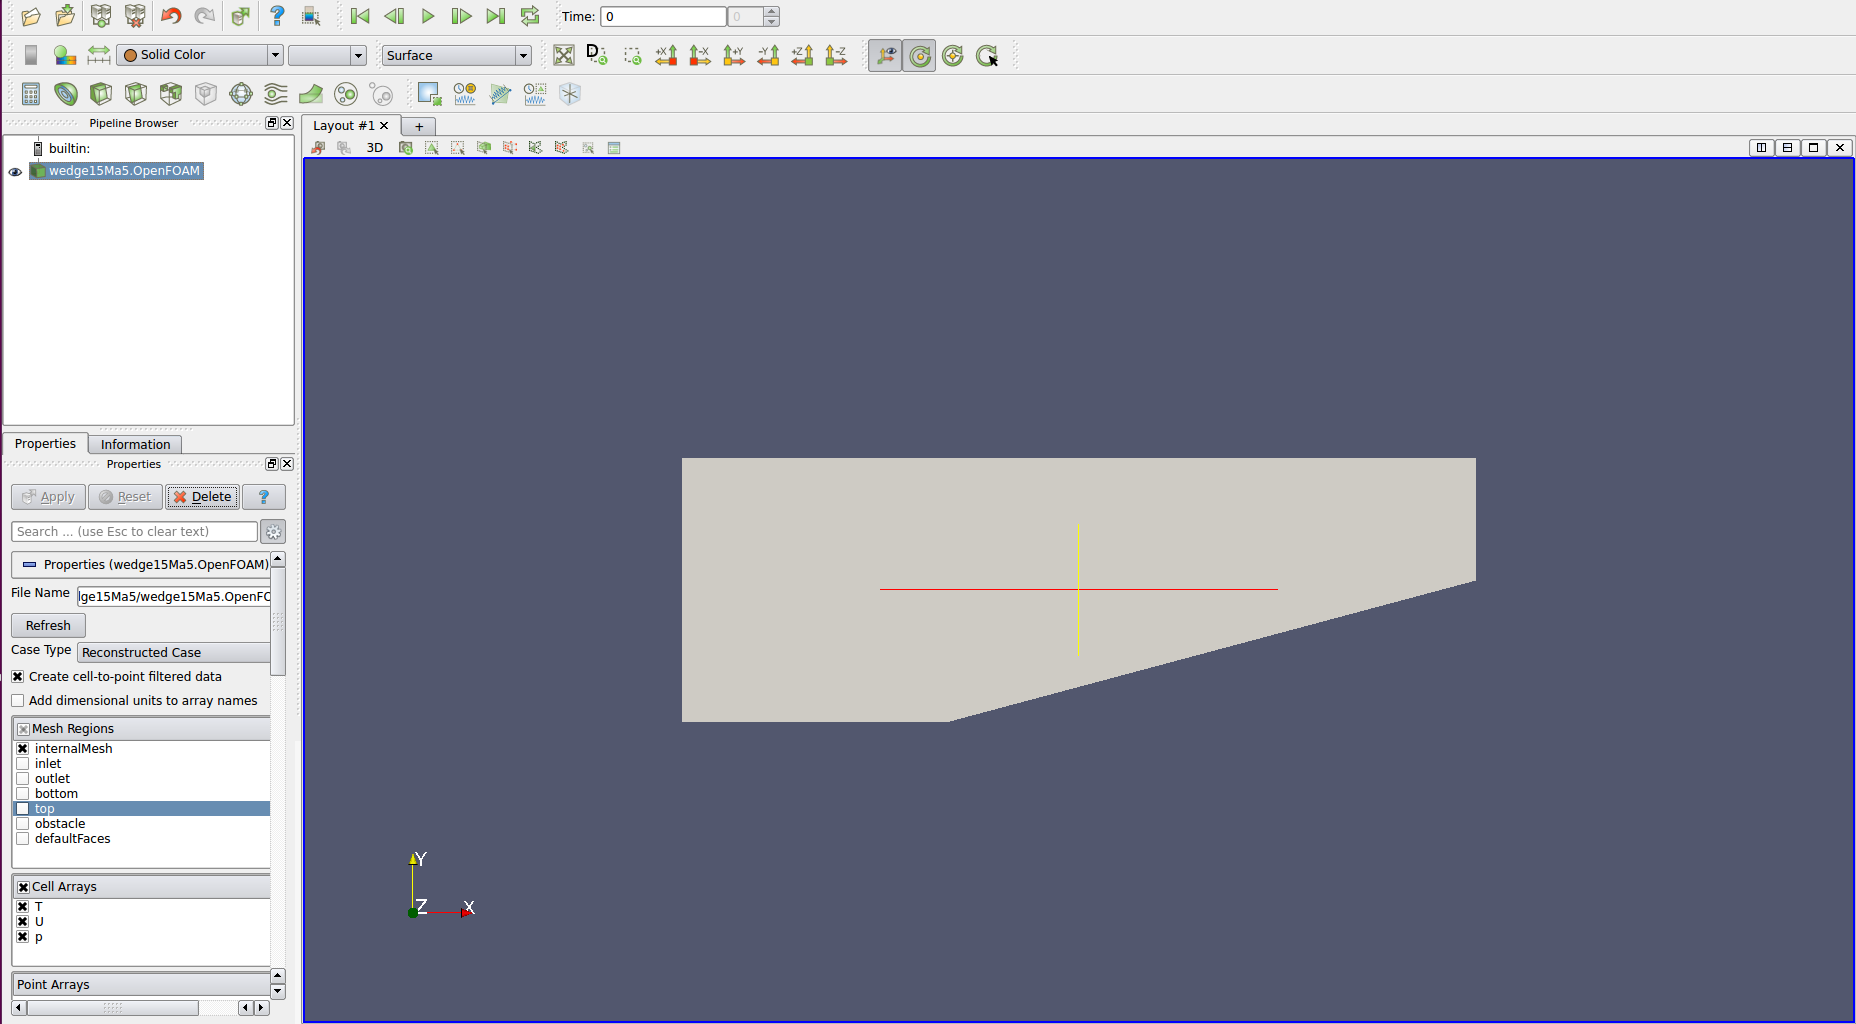
\includegraphics[scale=0.24]{\LocCHfivefig/para1.png}
\caption{Surface visualization of the 2-D wedge domain in ParaFView}
\label{para1}
\end{center}  
\end{figure}

\flushleft Now in the ParaView window you can check or uncheck the different regions within the 'mesh region' in  the Object Inspector Menu to visualize differnt regions on the geomtery. You can also visualize the geometry in wire-frame instead of surface by changing it from the down-down Active Variable Control Menu, to check out the quality of mesh.After inspecting the geomety you may close the ParaView window and switch back to the command terminal.

\begin{figure}[ht]  
\begin{center}  
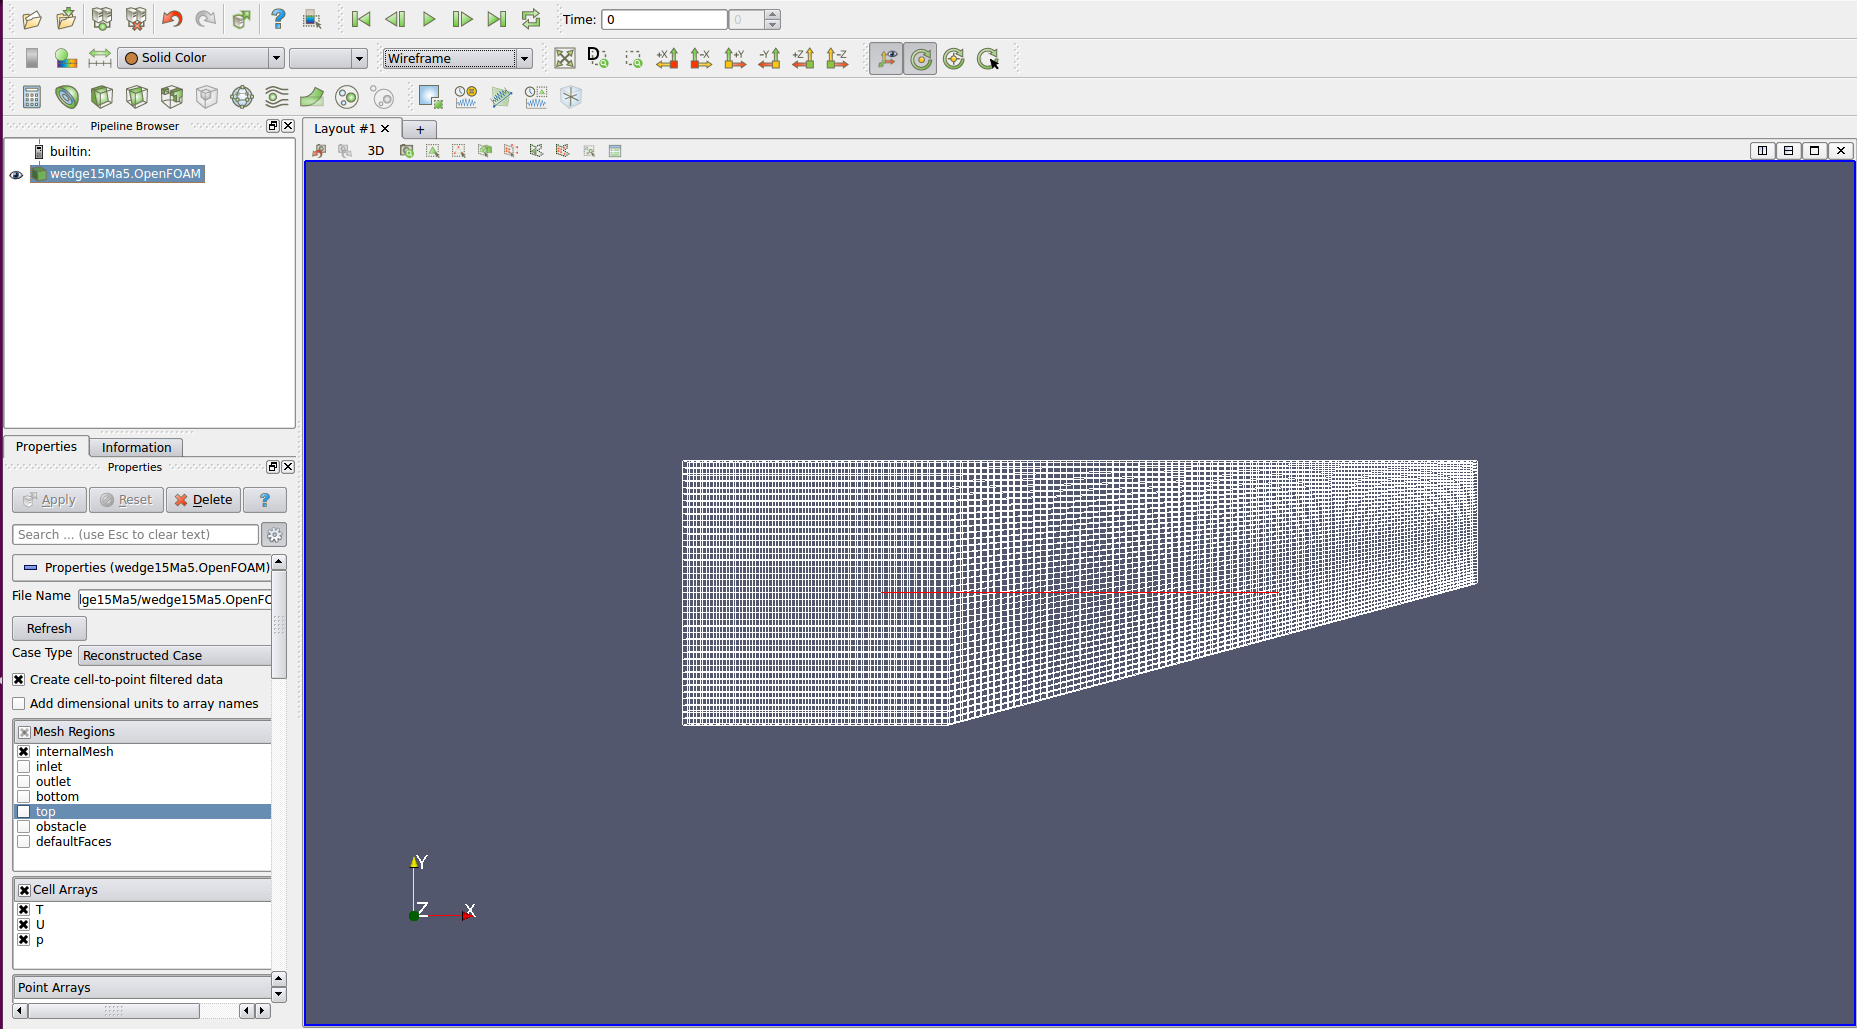
\includegraphics[scale=0.24]{\LocCHfivefig/para2.png}
\caption{Wireframe visualization of the 2-D wedge domain in ParaFView}
\label{para2}
\end{center}  
\end{figure}

\flushleft Now to run the solver switch back to the command terminal and type 'rhoCentralFoam' <enter>. The solver 'rhoCentralFoam' is a density-based compressible flow solver based on central-upwind schemes of Kurganov and Tadmor. You can see the progressing iterations in the terminal window along with the residual values. After the iteration ends type 'paraFoam' <enter> in the terminal window for post-processing.  
\flushleft This would open the ParaView window. As mentioned previously press apply on the left hand side of the Object Inspector Menu to view the new geometry. After this you can check or uncheck the different regions within the mesh region in  the Object Inspector Menu to visualize differnt regions on the geomtery. Now to check the velocity contours select U from the drop-down Active Variable Control Menu, from the visible toolbar. This will show the initial velocity countour of the cavity, as shown in fig \ref{velini}. Along with this you may also select the Toggle Colour Legend from the toolbar to visualize the legend. 

\begin{figure}[ht]  
\begin{center}  
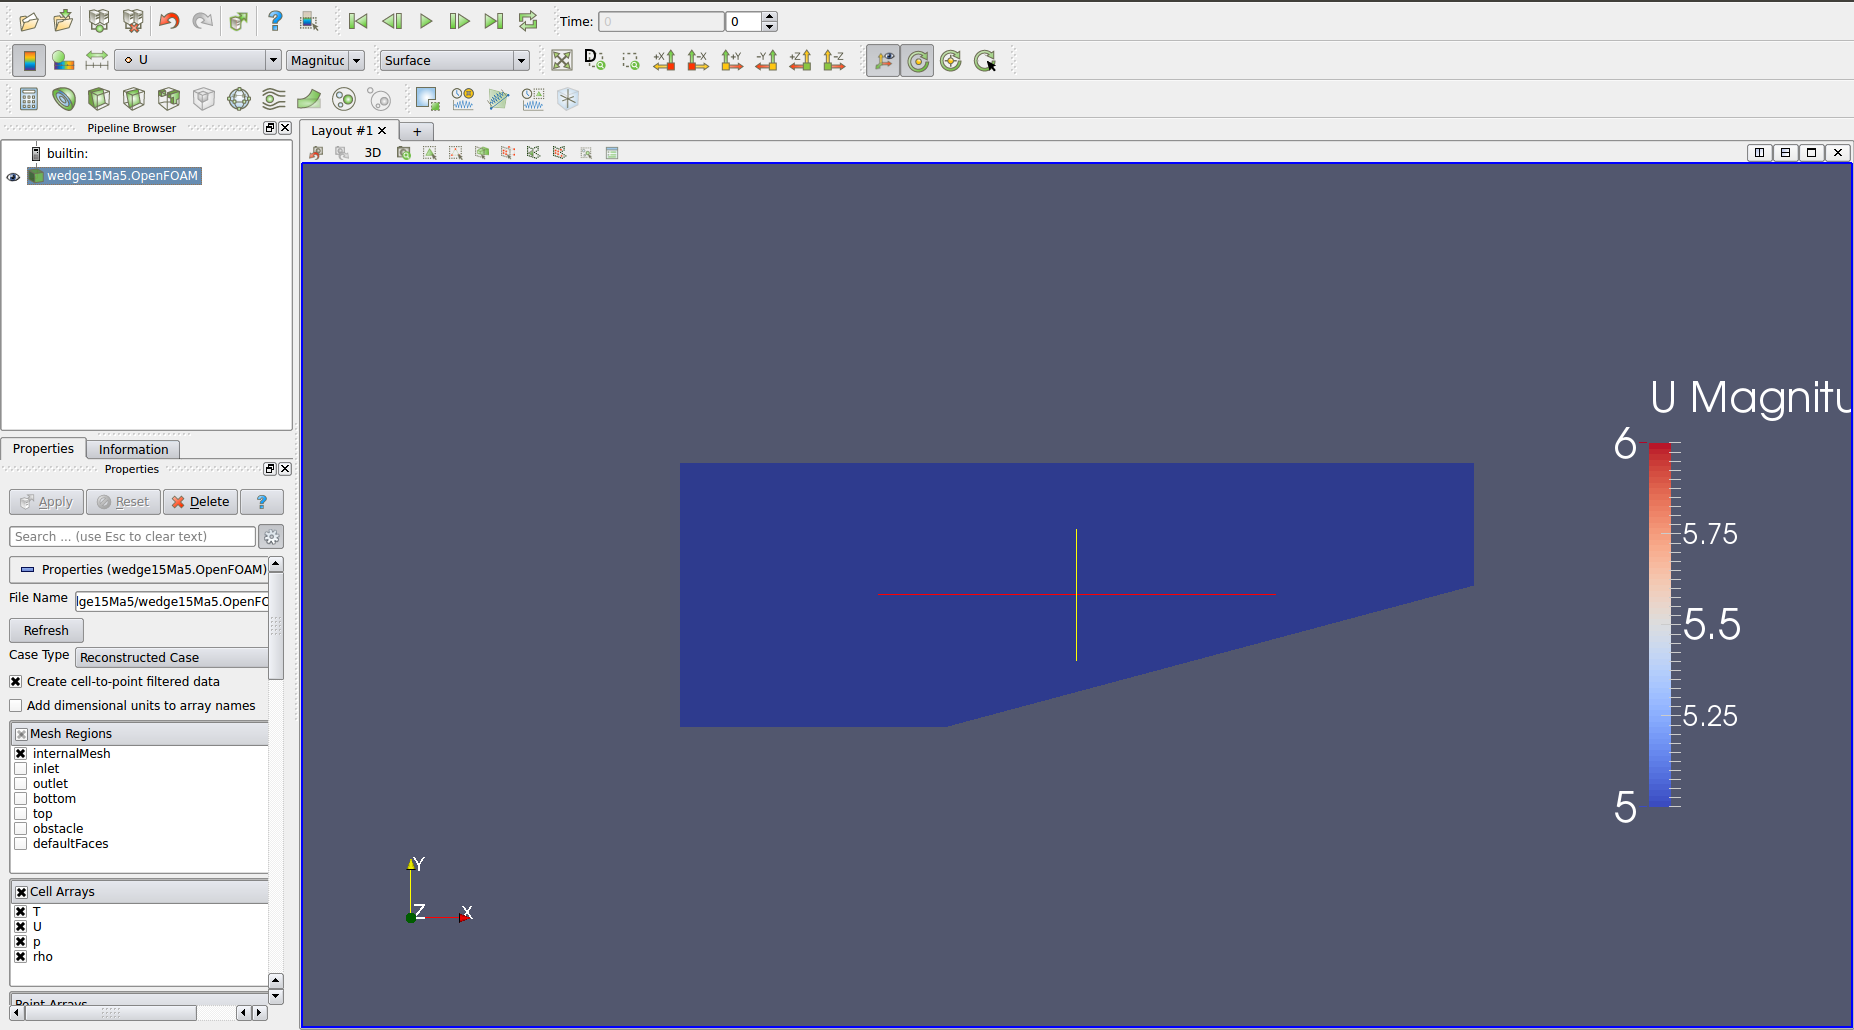
\includegraphics[scale=0.24]{\LocCHfivefig/velini.png}
\caption{Velocity contour in the 2-D wedge domain at initial state in ParaFView}
\label{velini}
\end{center}  
\end{figure}

\flushleft Now in the paraView window press the 'play' buttom from the VCR control. This would visualize the changing velocity countour along with the progressing iterations. You can see the final velocity contour as shown in fig \ref{vel}. Now on the ParaView window press apply on the left hand side of the Object Inspector Menu to view the meshed geometry. 

\begin{figure}[ht]  
\begin{center}  
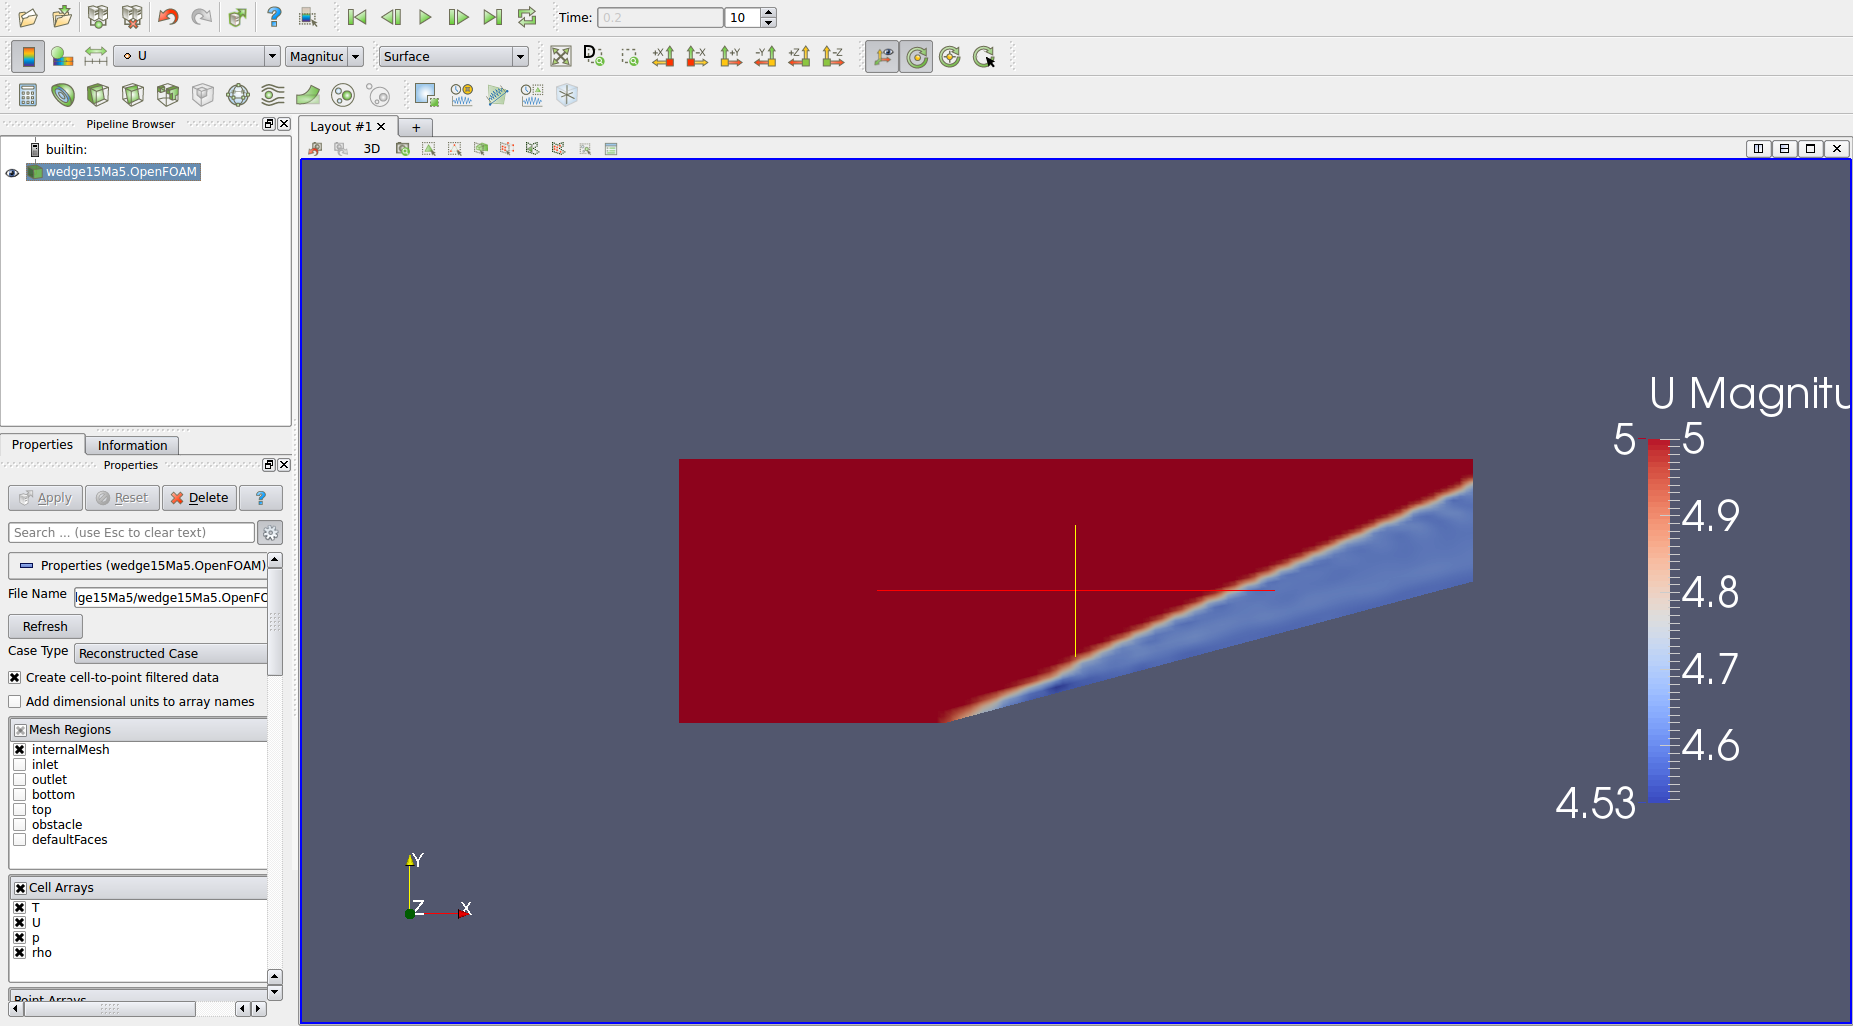
\includegraphics[scale=0.24]{\LocCHfivefig/vel.png}
\caption{Velocity contour in the 2-D wedge domain at final state in ParaFView}
\label{vel}
\end{center}  
\end{figure}

\flushleft Similarly, you can also plot the pressure and temperature contours.
\flushleft Now we can also calculate the mach number in this flow using a utility function in OpenFoam. To do this close the paraView window and switch to the command terminal. Here type 'Mach' and press $<$enter$>$. Note that “M” is capital here. This would calculate the Mach number in the flow for every time step.
\flushleft Now to view the Mach number contour type 'paraFoam' in the command terminal and press $<$enter$>$. Here select Mach in the left hand side properties window to include Mach number for post-processing. Now select 'Ma' from the drop-down Active Variable Control Menu, from the visible toolbar. And then press the play button on the VCR control toolbar. Along with this you may also select the Toggle Colour Legend from the toolbar to visualize the values to Mach number.
 %suba
%\input{CHAPTERS/chap6/chapter6.tex}
%\input{CHAPTERS/chap7/chapter7.tex}
%\input{CHAPTERS/chap8/chapter8.tex}
%\input{CHAPTERS/chap9/chapter9.tex}
\chapter{Downloading and Installing Salome}
\thispagestyle{empty}
\label{sec:chap10}
\newcommand{\LocCHtenfig}{\Origin/CHAPTERS/chap10/figures}

Salome is a Free and Open Source  CAD (Computer Aided Drawing), Meshing and Visualization Software for Numerical simulation. 
We can Create/modify, import/export (IGES, STEP, BREP), repair/clean CAD models and Mesh CAD models, edit mesh, check mesh quality, 
import/export mesh (MED, UNV, DAT, STL) using Salome. In this chapter we will learn how to download and intall Salome in any Operating system.

\section{Download Salome}

Open your browser and in the address bar type the url given below, \newline

\centering \textbf{www.salome-platform.org} \newline

\flushleft To Download Salome the user needs to create a account on the salome site. To do this on the left hand side of the salome screen website
scroll down to the bottom of the \textbf{Navigation} bar, Fig \ref{navi}, where you can see the new user option. Click on it and enter the required
personal details. \newline
\flushleft After you enter the details click on the register button at the bottom as shown in, Fig \ref{details}. Once done you will be directed 
to a screen showing that you have been registered. This also states thatv once you have done with registration you have to login to your email. Now 
open the mail sent by Salome and click on the link shown in Fig, \ref{link}. This link will direct you to a window where you need to set your password
for your Salome account. Enter the password and confirm it and press set my password button, Fig \ref{pass}. After this it will direct you to a window
which says your password has been set successfully. You may now login with your username and password. \newline

\flushleft In the Navigation bar click on Downloads after which you will be directed to a page which will show various bianaries for various Linux
distributions. You can choose according to your Operating System and 32/64 bit size. Since in this book we are working on a 64 bit platform we
will download Linux Debian 7 64-bits binary, Fig \ref{binary}. Click on it and Save the file. Downloading may take some time due to the large file size.
After this scroll down to Universal Binaries and click on the \textbf{Linux 64-bits} to download it. Note that 32-bit version of binaries are no
more supported for the latest version of Salome. \newline

\section{Installation}

Create a new folder in your home directory by the name Salome. Once these files are downloaded go to your Downloads folder and copy the tar file and a Self Extracting file and paste this inside your Salome folder. To extract the tar file right click on the tar file and select extract here. We can now see the extract wizard folder. \newline

Open a new terminal window and type in the path for the Installation Wizard folder in  the Salome folder of your home directory. \newline

\centering \textbf {cd /home/Salome/InstallationWizard\_7.6.0\_Debain\_64bits} \newline

\flushleft Type ls to view the content inside the file. An executable file by the name \textbf{runInstall} can be seen here. The Installation Wizard can be launched in two modes : GUI and Batch. The default installation settings can be overridden by using command line options. Each option has a short and a long notation. In the command line type : \newline

\centering \textbf{ ./runInstall [options]} \newline 

\flushleft Options include 

\begin{itemize}

\item -g / --gui : Runs the Installation Wizard in the GUI mode (this is the default mode).

\item -b / --batch : Runs the Installation Wizard in the terminal mode.

\end{itemize}

\flushleft Once the user has finished installation by either the GUI or Batch mode we now need to install the universal library. Since the binary is available in the same folder in the 
command terminal we can type : \newline 

\centering \textbf{ ./Salome-V7\_6\_0-LGPL-x86-64.run} and press enter \newline

\flushleft Enter the default path for the installation file. After this type N to use Salome in English.The installation prcocess now starts and might take a while. Close the terminal once this is done. Now you can see the Salome icon on your Desktop, Fig \ref{salome-icon}. Double click on this to open the Salome working window, Fig \ref{salome-win}. This brings us to the end of the chapter. In the next chapter we will learn more about how to create Geometries using Salome and using it for our OpenFOAM Simulation.



\begin{figure}[h]  
\centering
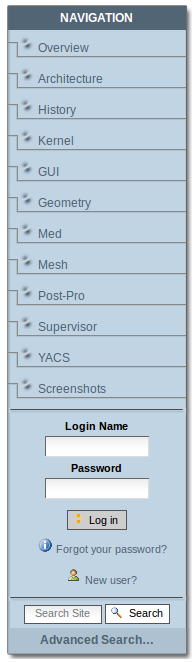
\includegraphics[scale=0.3]{\LocCHtenfig/navi.png}
\caption{Navigation Bar}
\label{navi}
\end{figure}

\begin{figure}[h]  
\centering
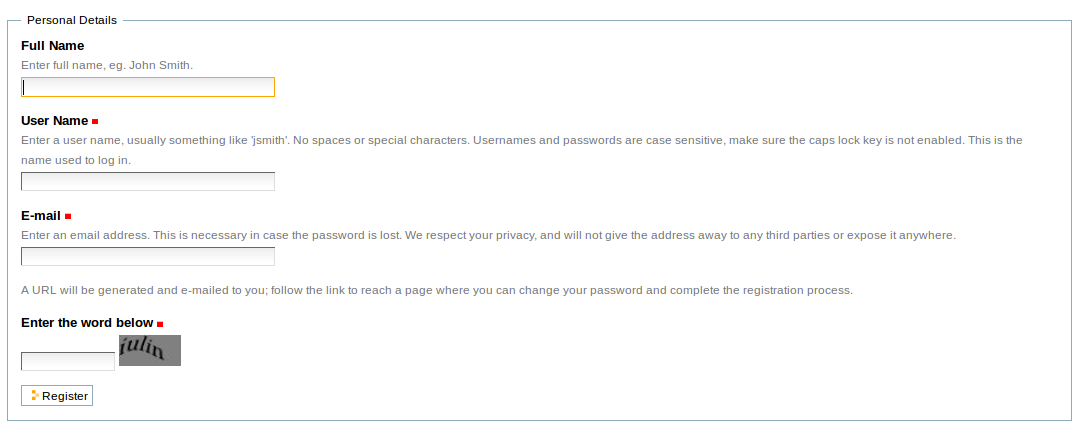
\includegraphics[scale=0.32]{\LocCHtenfig/details.png}
\caption{User Details}
\label{details}
\end{figure}

\begin{figure}[h]  
\centering
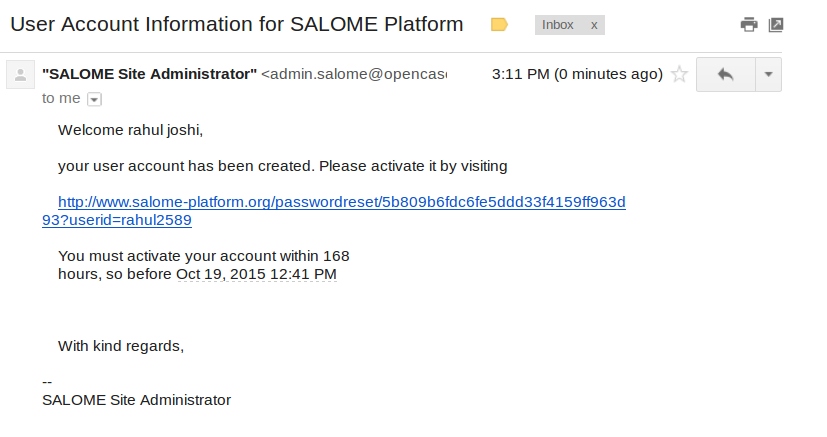
\includegraphics[scale=0.35]{\LocCHtenfig/link.png}
\caption{Salome Link}
\label{link}
\end{figure}

\begin{figure}[h]  
\centering
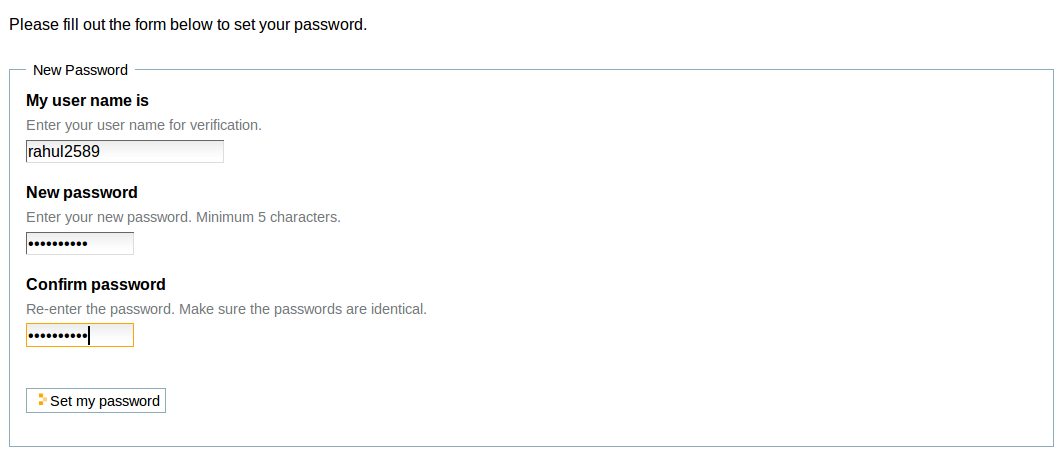
\includegraphics[scale=0.35]{\LocCHtenfig/pass.png}
\caption{Enter Password}
\label{pass}
\end{figure}

\begin{figure}[h]  
\centering
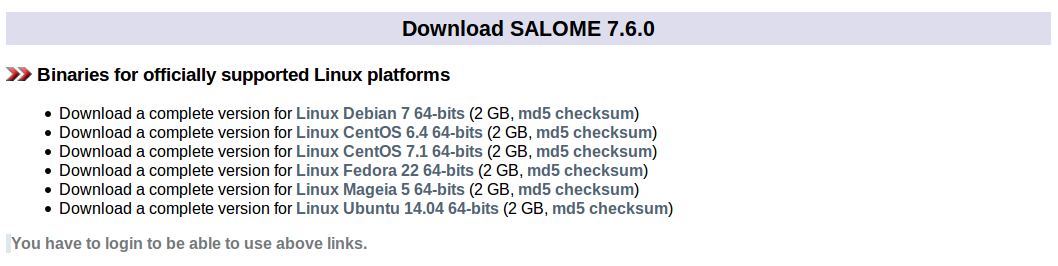
\includegraphics[scale=0.35]{\LocCHtenfig/binary.png}
\caption{Salome Linux 7 64 bit binary}
\label{binary}
\end{figure}

\begin{figure}[h]  
\centering
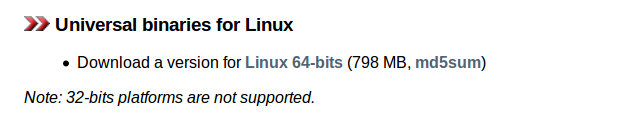
\includegraphics[scale=0.35]{\LocCHtenfig/universal.png}
\caption{Universal Binaries}
\label{univ}
\end{figure}

\begin{figure}[h]  
\centering
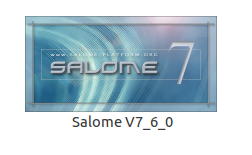
\includegraphics[scale=0.35]{\LocCHtenfig/salome-icon.png}
\caption{Salome icon}
\label{salome-icon}
\end{figure}

\begin{figure}[h]  
\centering
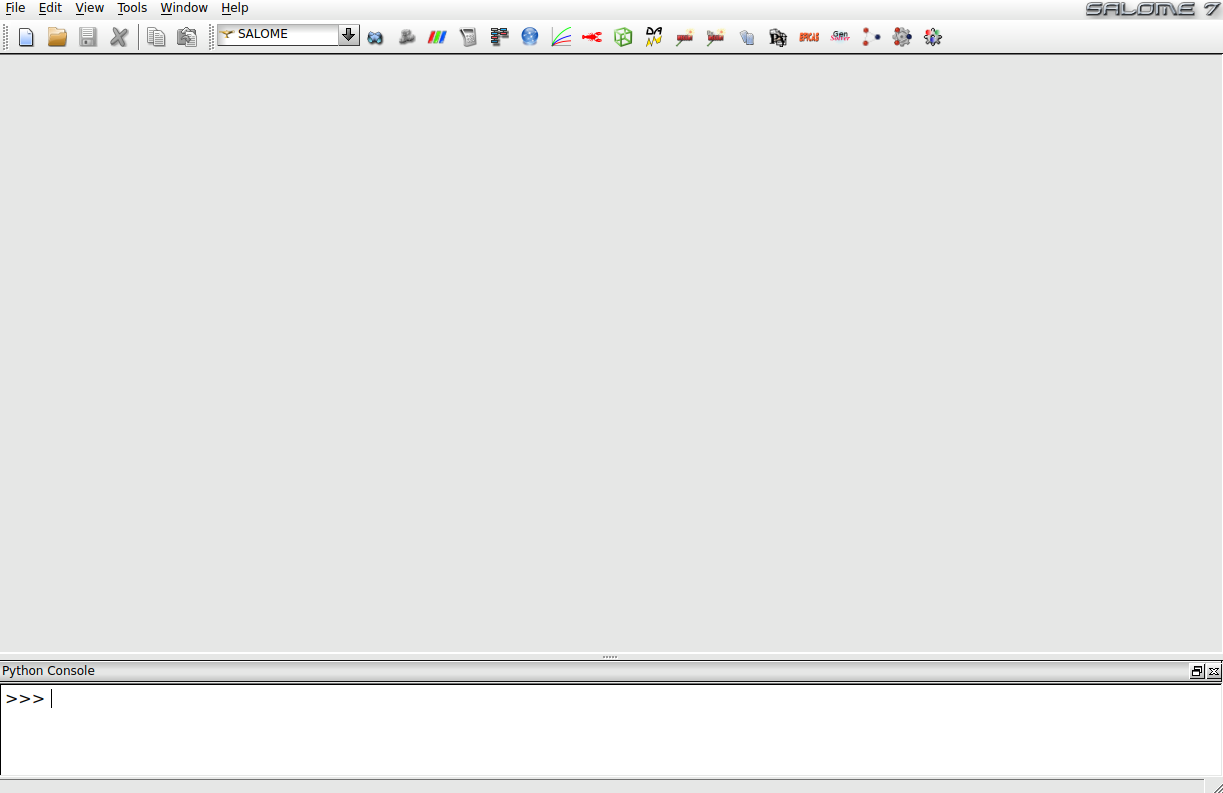
\includegraphics[scale=0.25]{\LocCHtenfig/salome-win.png}
\caption{Salome working window}
\label{salome-win}
\end{figure}
 %rahul
%\input{CHAPTERS/chap11/chapter11.tex}
%\chapter{Exporting geometry from Salome to OpenFOAM}
\thispagestyle{empty}
\label{sec:chap12}
\newcommand{\LocCHtwelvefig}{\Origin/CHAPTERS/chap12/figures}

A 90 deg pipe bend is perhaps the most frequent used fitting in piping systems. The pressure losses in such bends are therefore of considerable engineering importance. This chapter is extension of the the chapter number, where we learnt about creating and meshing a curved pipe in Salome, hence it is manditory that the learner should have already gone through the previous chapter . In this chapter we will learn how to group the mesh faces in Salome, save the mesh file and export the mesh file to be used in OpenFOAM. Here we will also create a case directory to solve this problem and visualize the results in Paraview. \newline

Open the salome working window as shown in the previous chapters. Click on the File in the menu bar and click on Open. Now go to the path where you had saved your geometry in the previous chapter i.e. \textbf{"$*$.hdf"} and open it. \\

Since we have already meshed our geometry will will skip the geometry module and select the Mesh module from module drop down menu. Module $>>$ Mesh. In the object browser we can see the Mesh module, click it to expand the Mesh module tree. Here we will see Mesh_1. The meshed geometry will not be visible in the Salome working window. To view the meshed geometry , right click on Mesh_1 and click on Show. The meshed geometry can be seen as shown in figure, \ref{mesh_1}. Once we open the mesh we will start to group it so that we can export it and use this in OpenFOAM. 

\begin{figure}[h]  
\centering
\includegraphics[scale=0.35]{\LocCHelevenfig/mesh_12_1.png}
\caption{Meshed geometry in Salome working window}
\label{mesh_1}
\end{figure}   

\section{Creating Groups}

In Mesh we can create a group of elements of a certain type. This helps us to identify the boundary patches in OpenFOAM. To create group from the top menu bar click on "Mesh" and slect "Create Group" To create a group once needs to define the following, \newline
\begin{itemize}
\item Mesh - The mesh from which elements will be selected to form the group. We can select the mesh in the Object Inspector Menu or in the 3D viewer.
\item Element type - These are a set of radio buttons which allows us to select the type of element which will form the group.
\begin{itemize}
\item Nodes
\item 0D elements
\item Ball
\item Edges
\item Faces
\item Volumes
\end{itemize}
\item Name - this field allows you to enter the name of the new group eg, "inlet"
\item Color - assigns color to a certain group. This helps to display the elements of a group
\item We can also distinguish between three group type as Standalone geometry, Group on geometry and group on filter.
\end{itemize}

\section{Grouping Mesh}
Since we have three patches in our geometry we will select the "Face" option from create groups and Group on geometry as the group type, this is because we will be grouping the elements of a certain type generated on our geometry. The Group on Geometry can be created only if the mesh is based on geometry. To define a group we choose the Group on geometry check box and then click the selection button besides Gemetrical object as shown in the figure \ref{mesh_1}. 

\begin{figure}[h]  
\centering
\includegraphics[scale=0.35]{\LocCHelevenfig/mesh_12_1.png}
\caption{Meshed geometry in Salome working window}
\label{mesh_1}
\end{figure} 

Here we get two options
\begin{itemize}
\item Direct geometry selection - to select a shape in the Object Browser 
\item Find geometry by mesh element selection - to activate a dialog which retrives a shape by the selected element generated on this shape.
\end{itemize} //

We will use direct geometry selection since we have already grouped our geometry while creating the geometry. Open the geometry tree in the object browser and click on the Pipe$\_$1 and select the group which we had created during geometry such as "inlet", "outlet" and "walls". These faces can be identified by color by selecting a color from Color group . We can give names to this group of our choice , in this chapter we have kept the same name as that given in geometry i.e. "Inlet".Finally click on Apply and close to end the geometry selection. Follow the similar procedure for naming outlet faces of the mesh. Inlet and Outlet group will be seen in the Mesh-1 tree. For selecting the faces for walls we select the element type in Create group as Face and Group type as Group on Filter. Now we click on the set filter.This open a new box named as Filter for faces \ref{mesh_1}, click on the "Add" button. In the drop down menu below Criterion select "Free faces" and click on Apply and close. You can provide any color of your choice here. Click on Apply and close to create Group-1. From the menu bar now click on Mesh menu and select Cut of groups and select the main object as Group-1 as shown in figure \ref{mesh_1}. Click on tool object and from grouped object select Inlet, hold the shift key and select Outlet. We can see the Result name on top of the window, type "walls". Select any color of your choice and click on Apply and close. This will now create a group named "walls" in the Mesh tress in object browser. Delete the Group-1 in the mesh tree as we no longer need the group. We can save our work by clicking on the Save Document option just above object browser. To export the mesh file right click on Mesh-1 and select Export and click on UNV file. Name this file as "bentpipe" and save it in your working directory. Now we can close salome.

\section{Creating Case directory}

To solve this problem in OpenFOAM we need to first create a case directory in OpenFOAM. We will be using icoFoam solver to solver this problem, which is an incompressible transient solver for laminar flows. We create a directory inside icoFoam and name it as bentpipe. Copy the bentpipe.unv file which we had saved and paste this into the bentpipe folder. Now Copy the 0 and system folder from the cavity folder to the bentpipe folder. The directory structure of the bentpipe folder is as shown in the figure, \ref{mesh_1}.

\begin{figure}[h]  
\centering
\includegraphics[scale=0.35]{\LocCHelevenfig/mesh_12_1.png}
\caption{Meshed geometry in Salome working window}
\label{mesh_1}
\end{figure}

Note that, we have not copied the constant folder here as it will be created once we have converted our mesh file from UNV to Foam format. Open the terminal window and type the path for bentpipe inside the icoFoam solver as follows \\
\centering{/OpenFOAM/OpenFOAM-2.x.x/tutorial/incompressible/icoFoam/bentpipe}

\subsection{Geometry conversion}

To convert the geometry from UNV format to OpenFOAM recognisable format we use the command as shown below, \\

\centering{ideasUnVToFoam -filename}

The file name in our case would be bentpipe.unv. Once the file is converted we can see that the constant folder is created. The polyMesh folder inside constant folder stores the information regarding geometry, check this folder for files such boundary, faces, neighbours, owner, points. Also do not forget to copy the transportProperties file from the cavity folder and paste this inside the constant folder

\subsection{Geometry Scaling}     

In Salome, by default the geometry is created in millimeters. To convert the geometry from millimeters to centimeters we will use the OpenFOAM utility of transformPoints. In In the command terminal type  the command given below for using this utility and press enter\\

\centering{transformPoints -scale '(0.01 0.01 0.01'}

We will see that the geometry has been converted to centimeters.

\section{Setting 0 folder}

As we had copied the 0 folder from the cavity case we need to make changes inside the pressure (p) and Velocity (U) file for matching the boudnary names given in Salome. Open each file and insert the boundary name and boundary condition as shown in the table below for both pressure and velocity.


\section{Visualization}

The case directory tress for the bentpipe case will be as shown below, \ref{mesh_1}.

\begin{figure}[h]  
\centering
\includegraphics[scale=0.35]{\LocCHelevenfig/mesh_12_1.png}
\caption{Meshed geometry in Salome working window}
\label{mesh_1}
\end{figure}

To visualize the geometry we will open Paraview using the paraFoam command in terminal.Click on Apply button in the Object Inspector menu, we will see the geometry as seen in the figure \ref{mesh_1}.

\begin{figure}[h]  
\centering
\includegraphics[scale=0.35]{\LocCHelevenfig/mesh_12_1.png}
\caption{Meshed geometry in Salome working window}
\label{mesh_1}
\end{figure}

Now to view the mesh , from the drop down menu select Surface with Edges. Zoom into the geometry to see the mesh. In Mesh parts inside Object Inspector we can see that the groups have been properly created and match with that created in Salome namely "Inlet", "Outlet" and "Walls". Volume of pipe by default is named as "internalMesh". This bring us to the end of this chapter.

\section{Assignment}

In this chapter and the earlir chapter 11, we have seen how to create geometry, mesh the geometry and create groups for the mesh file to be imported inside OpenFOAM. As an assignment create a bentpipe with radius 5 mm and total length of 300 mm and export the geometry in "unv" file format. Finally visualize the results in OpenFOAM.
%\input{CHAPTERS/chap13/chapter13.tex}
%\input{CHAPTERS/chap14/chapter14.tex}
\chapter{Importing Mesh From Third Party Software in OpenFOAM}
\thispagestyle{empty}
\label{sec:chap15}
\newcommand{\LocCHonefivefig}{\Origin/CHAPTERS/chap15/figures}

OpenFOAM can be used for creating and meshing geometrical shapes like Box, Pipe. When dealing with complex geometries like a turbine blade, aircraft,
ship etc, we cannot use the blockMesh utility. In such cases it is always better to create the geometry and mesh in dedicated CAD and Meshing softwares 
and solve those usiing OpenFOAM. As a prerequisite it is expected the user should have knowledge about creating geometry and generating mesh in softwares
like Gmabit, Gmsh, Salome, ICEM etc. This chapter deals with the steps involved in importing mesh files in OpenFOAM using different mesh conversion tools.

\section{Geometry}

We will use the above problem of Flow over a square cylinder as an example for importing mesh file in OpenFOAM. Here we have a square cylinder
of length 1m and height 1 m. Inlet velocity is set at 1 $\frac{m}{s}$ for Reynolds number (Re) 100. The size of the domain choosen is 60 m by 40 m.
The boundary conditions are as shown in the , Fig \ref{square} below.

\begin{figure}[t]  
\centering  
\includegraphics[width=\lgfig]{\LocCHonefivefig/square.png}
\caption{Flow over square Cylinder}
\label{square}  
\end{figure}

\section{Meshing}

We have generated a hexhedral mesh for the above geometry with 40000 cells and saved the mesh file as cylmesh.msh. 
The mesh generated is as shown below, Fig \ref{mesh} 

\begin{figure}[h]  
\centering
\includegraphics[width=\lgfig]{\LocCHonefivefig/cylmesh.jpeg}
\caption{Mesh}
\label{mesh}
  
\end{figure}

\section{Importing the mesh file}

In incompressibel solvers go to icoFoam and create a solver inside it by the name \textbf{cylinder}. Now go inside the cavity case and copy the 
\begin{itemize}
\item 0
\item system
\end{itemize}

\flushleft folder and paste it inside the cylinder folder. Please make a not here that we do not need the \textbf{constant} folder here. After this copy the 
cylmesh.msh mesh file create earlier and paste this inside this folder. Thus the our case file is now ready. Now open the command terminal and type the
path for the cylinder folder. Now since we have a Fluent (.msh) mesh file we will use the mesh conversion command as shown below followed by the file name \\
\centering \textbf{fluentMeshToFoam file-name.msh} \newline

\flushleft In the terminal window type the above command with the file name and press enter.

\begin{figure}[h]  
\centering
\includegraphics[width=\lgfig]{\LocCHonefivefig/conversion.png}
\caption{convert}
\label{mesh}
\end{figure}

\flushleft In case you have a 3D mesh file then you can use the command \\ \vspace{0.5cm}
\centering {\textbf{fluent3DMeshToFoam file-name.msh}} \newline

\flushleft The Fluent mesh file is converted into OpenFOAM mesh file. Now if we look back into our cylinder folder we can see that the "constant"
folder is now generated. When we open the constant folder we will see that the transport properties file is missing. Since we had converted the 
fluent mesh file into openfoam the fluid property files were missing. Copy the transport property file from the constant folder of cavity case
and paste this inside the constant folder of cylinder. The trasnportProperties file contains the value of fluid viscosity, we can either change it
or keep it default. \newline

\flushleft Make a note here that we do not use the \textbf{blockMesh} command here

\section{Boundary Conditions}

When we import the geometry in OpenFOAM we need to be very careful with the boudnary names used while creating the mesh file. Since OpenFOAM is case
sensitive in case of any mistake with the boundary names can create an error while running the solver. To view the boundary names in the command terminal
go to polyMesh folder inside the constant. Inside polyMesh you can see a file by the name \textbf{boundary}. Open this file in any editor of your
choice, eg, gedit boundary, Fig \ref{boundary}.

\begin{figure}[h]  
\centering
\includegraphics[width=\lgfig]{\LocCHonefivefig/boundary.png}
\caption{Boundary file}
\label{boundary}
\end{figure}

\flushleft The boundary names will be as shown in the domain shown above, Fig \ref{square}. In case of any error with the boundary names you can
always refer to this boundary file. Now in your command terminal go to the 0 folder and open the pressure file. Make sure that the boundary names 
match exactly the names in the boundary file, in case of errors make the necessary changes.

\section{Solver settings}

In the terminal window go to the controlDict file inside system and open it in any editor of your choice. Change the endTime from 0.5 to 1.5 seconds.
Save the file and close it, Fig \ref{cd} and come back to the cylinder folder.

\begin{figure}[h]  
\centering
\includegraphics[width=\lgfig]{\LocCHonefivefig/controldict.png}
\caption{controlDict file}
\label{cd}
\end{figure}

\flushleft After making the necessary changes we can now run the solver. In the temrinal window type the name of the solver \textbf{icoFoam}
and press enter. The iterations will be seen running on the terminal window. After the iterations stop we can now start with the visualization.

\section{Post-Processing}

Launch paraview by typing \textbf{paraFoam} in the terminal window and once it opens click on the Apply button to view the geometry, Fig \ref{geom}.
In the active varialble control menu change from Solid Color to Velocity (U). You can now see the initial conditions for velocity, Fig \ref{vel}.
To view the animation on the right hand top of paraview click on the play button of VCR menu. You can see the change in velocity in the paraview 
window with the passage of time, Fig \ref {vel-1}.

\begin{figure}[h]  
\centering
\includegraphics[width=\lgfig]{\LocCHonefivefig/geom-paraview.png}
\caption{Geometry in Paraview}
\label{geom}
\end{figure}

\begin{figure}[h]  
\centering
\includegraphics[width=\lgfig]{\LocCHonefivefig/vel.png}
\caption{Initial velocity condition}
\label{vel}
\end{figure}

\begin{figure}[h]  
\centering
\includegraphics[width=\lgfig]{\LocCHonefivefig/vel-1.png}
\caption{Velocity at 1 sec}
\label{vel-1}
\end{figure}

\section{Mesh Conversion Commands}

The user can also import mesh files from other meshing softwares as well. Here is a list of commands to import mesh files in OpenFOAM.

\begin{itemize}
\item ANSYS : ansysToFoam file-name
\item IDEAS : ideasToFoam file-name
\item CFX : cfxToFoam file-name
\item SALOME : ideasUnvToFoam file-name
\end{itemize}


 %rahul
\chapter{Installing and Running Gmsh}
\thispagestyle{empty}
\label{sec:chap16}
\newcommand{\LocCHonesixfig}{\Origin/CHAPTERS/chap16/figures}

Gmsh is a Free and Open Source three dimensional finite element grid generator with a build-in CAD engine and post-
processor. There are four modules available in Gmsh such as Geometry, Meshing, Solver and Post-Processiing. The specification 
of any input to these modules is done either interactively using the graphical user interface or in ASCII text files using its own scripting language.
With Gmsh we can create and mesh a geometry and import it in OpenFOAM or import a CAD file (stl, step) and use it for OpenFOAM using the mesh conversion utilities (see chapter 17 for more info).
In this chapter we will cover how to install Gmsh and create a simple geometry.It is expected that the user should have knowledge 
about Meshing.

\section{Installing Gmsh}

Gmsh can be installed using Synaptic Package Manager. Open Gmsh in your system by typing your system password.
In the search box type Gmsh and install it, Fig \ref{synaptic-gmsh}. This might take some time depending on your internet speed.

\begin{figure}[ht]  
\begin{center}  
\includegraphics[scale=0.32]{\LocCHonesixfig/synaptic-gmsh.png}
\caption{Install Gmsh}
\label{synaptic-gmsh}
\end{center}  
\end{figure}


\flushleft Alternately we can also install Gmsh from the gmsh website given below,

\center {\textbf{http://geuz.org/gmsh/}} \newline

\flushleft Open this website in your browser and scroll down to download. Now Download Gmsh according to the given current stable release 
Fig \ref{download-gmsh} according to your Operating System (OS).

\begin{figure}[ht]  
\begin{center}  
\includegraphics[scale=0.352]{\LocCHonesixfig/download-gmsh.png}
\caption{Download stable release}
\label{download-gmsh}
\end{center}  
\end{figure}

\begin{figure}[ht]  
\begin{center}  
\includegraphics[scale=0.26]{\LocCHonesixfig/gmsh-icon.png}
\caption{gmsh-icon}
\label{gmsh-icon}
\end{center}  
\end{figure}

\section{Running Gmsh}

\flushleft In the Download folder extract the downloaded gmsh tar file. After you open the folder you will see folder named bin, click on it. 
Inide the bin folder you will see the Gmsh icon, Fig \ref{gmsh-icon}. Double click on it to launch the Gmsh Start screen, Fig \ref{gmsh-start} \newline

As a pracice to learn Gmsh we will create a cube of sides 1 unit as seen in the Fig, \ref{geometry1}. On the left hand side in the Gmsh window you can 
see three modules namely,

\begin{itemize}
\item Geometry
\item Mesh
\item Solver
\end{itemize}

Click on the Geometry module, then go to Elementary Entities, inside elementary entities go to add and then click on points. This will open up a
window where you can enter the X, Y and Z co-ordinates starting with 0 inside each box and press Enter, Fig \ref{point}. Now
enter points for all the remaining 7 vertices to complete the cube, Fig \ref{geometry1}. In the Gmsh screen we can see the eight points, you can move those points
using the left mouse click. To join these points click on Straight-line option under Elementary Entities. Now select any two points to create a straight line, click 
on the start point and then the second point to create a line. Similarly join all the other points to create a cube as shown in the Fig, \ref{line} below.
As you can see on the Gmsh screen you can press e to end selection and q to abort.

\begin{figure}[t]  
\begin{center}  
\includegraphics[scale=0.28]{\LocCHonesixfig/gmsh-start.png}
\caption{Gmsh Start window}
\label{gmsh-start}
\end{center}  
\end{figure}

\begin{figure}[t]  
\begin{center}  
\includegraphics[scale=0.28]{\LocCHonesixfig/geometry1.png}
\caption{Geometry for Gmsh}
\label{geometry1}
\end{center}  
\end{figure}

\begin{figure}[t]  
\begin{center}  
\includegraphics[scale=0.28]{\LocCHonesixfig/point-gmsh.png}
\caption{Points window}
\label{point}
\end{center}  
\end{figure}

\begin{figure}[t]  
\begin{center}  
\includegraphics[scale=0.28]{\LocCHonesixfig/cube-gmsh.png}
\caption{Join points using line}
\label{line}
\end{center}  
\end{figure}

\subsection{Create Faces}

To create faces for the cube click on plane-surface unde elementery enetities. After this select the outer booundaries of the face of a rectangle.
Select the edges of the bottom face first.Once you select the edges they will turn red in color, Fig \ref{face}. Check in case if there is any hole in the 
face, if none then press e to end selection. You will notice that a face will appear with dasshed center lines, Fig \ref{cl}. Repeat this procedure for 
remaining faces, Fig \ref{face-all} and finally press q to abort.

\begin{figure}[t]  
\begin{center}  
\includegraphics[scale=0.28]{\LocCHonesixfig/face-red.png}
\caption{Selct edges}
\label{face}
\end{center}  
\end{figure}


\begin{figure}[t]  
\begin{center}  
\includegraphics[scale=0.28]{\LocCHonesixfig/face-cl.png}
\caption{Bottom Face}
\label{cl}
\end{center}  
\end{figure}

\begin{figure}[t]  
\begin{center}  
\includegraphics[scale=0.28]{\LocCHonesixfig/face-all.png}
\caption{Create faces for all surfaces}
\label{face-all}
\end{center}  
\end{figure}

\subsection{Creating Volume}

We now need to create volume boundary. We need to select the Volume boundary similar to selecting boundary for faces. 
Click on the Volume boundary under elementery entities and click on boundary surface of the cube and press e to end selection. A yellow dot will
appear at the center of the cube which represents volume in Gmsh. Press q to abort the selction.

\begin{figure}[t]  
\begin{center}  
\includegraphics[scale=0.28]{\LocCHonesixfig/vol-gmsh.png}
\caption{Volume}
\label{vol}
\end{center}  
\end{figure}

\subsection{Physical Groups}

Physical groups heps us to identify a set of points, lines, faces, volume with a unique Identification number. We create physical groups which will be useful for exporting the Mesh file to OpenFOAM.To do so click on Physical Group under Geometry Module. Click on Add and then Surface. Upon selection of any face it will turn red. Now press e to end selection. Do this procedure for all the remaining facesand press q to abort. Also we need to select the Physical Volume. Click on Volume under Physical Groups and select the yellow dot at the center of the cube.The yellow dot will turn red in colour adn press e to end selection and q to abort.

To save the geometry under the file menu click on Save as and save the geometry by the name cube.geo. Here "geo" stands for geometry. Click OK twice
to save the geometry. 
 %rahul
\chapter{Creating a Sphere using Gmsh}
\thispagestyle{empty}
\label{sec:chap17}
\newcommand{\LocCHonesevenfig}{\Origin/CHAPTERS/chap17/figures}

In the earlier chapter we learnt about how to Install and Run Gmsh by creating a simple geometry. As the earlier tutorial shows about basic geometry construction in Gmsh the user is expected to know it before starting this chapter. This chapter deals with creating a Sphere using Gmsh and meshing it. The chapter we will focus on creating the spherical geometry and the domain surrounding it and in the next chapter we will look into how to mesh this geometry. Since this is a spherical geometry we will learn about how to create a circular arc, how to create ruled surface and doing basic manipulation with the .geo file which generated. 

\section{Points}

You can start Gmsh by either double clicking on the gmsh-icon or from the terminal by typing \textbf{gmsh sphere1.geo} , this will open up the gmsh window. The first step after starting Gmsh is to mark the co-ordinates for our sphere, we define the center of the Sphere and points surrounding it. Co-ordinates for the sphere ( 7 points ) are as given below : \newline

\begin{itemize}

\item (0, 0, 0)
\item (-1, 0, 0)
\item (1, 0, 0)
\item (0, -1, 0)
\item (0, 1, 0)
\item (0, 0, -1)
\item (0, 0, 1)

\end{itemize}

\flushleft The points will appear on the Gmsh window as shown in the Fig \ref{points} below.

\begin{figure}[h]  
\centering
\includegraphics[scale=0.25]{\LocCHonesevenfig/gmshpts.png}
\caption{Sphere coordinates}
\label{points}
\end{figure}

\section{Circular Arc}

Creating an Arc is a three step process where we a start point, center and an end point . An important point to be noted here is that in Gmsh a Circular Arc is strictly created less than pi. Now to create an circular arc select Circle Arc option in the left hand side menu of Gmsh under Add. Click on the right most point in the Gmsh Window, it will turn red in colour, Fig \ref {point1}.

\begin{figure}[h]  
\centering
\includegraphics[scale=0.25]{\LocCHonesevenfig/point1.png}
\caption{Rightmost point}
\label{point1}
\end{figure}

\flushleft Now click on the center of the Sphere as shown in Fig \ref{point2} and that too will turn red in colour.

\begin{figure}[h]  
\centering
\includegraphics[scale=0.25]{\LocCHonesevenfig/point2.png}
\caption{Center of the sphere}
\label{point2}
\end{figure}

\flushleft For the end point click on the point above the center. As soon as we click on this point a arc is created as shown in the Fig \ref{point3}.

\begin{figure}[h]  
\centering
\includegraphics[scale=0.25]{\LocCHonesevenfig/point3.png}
\caption{End point of the Arc}
\label{point3}
\end{figure}

\flushleft Repeat this process for all the points to complete the sphere. Create the Arcs keeping the same center point. The completed geometry of the sphere is as shown , Fig \ref{}

\begin{figure}[h]  
\centering
\includegraphics[scale=0.25]{\LocCHonesevenfig/sphere.png}
\caption{Sphere}
\label{sphere}
\end{figure}

\section{Surface Creation}

To stich the arcs together we now need to create surfaces. To do so, click on the Ruled Surface option under Add menu. Now select bounding edges for the surface as shown in Fig \ref{surface}. After the selction they will turn red in colour. Press e on your keyboard to execute this selection. A crossed dotted line will be visible which shows that the surface has been created, Fig \ref{surf1}. Repeat the process to create all eight surfaces of the sphere, Fig \ref{surf2}.

\begin{figure}[h]  
\centering
\includegraphics[scale=0.25]{\LocCHonesevenfig/surface.png}
\caption{Surface Bounding edges}
\label{surface}
\end{figure}

\begin{figure}[h]  
\centering
\includegraphics[scale=0.25]{\LocCHonesevenfig/surf1.png}
\caption{Surface Creation}
\label{surf1}
\end{figure}

\begin{figure}[h]  
\centering
\includegraphics[scale=0.25]{\LocCHonesevenfig/surf2.png}
\caption{Complete Surface Creation}
\label{surf2}
\end{figure}

\section{Editing .geo file}

Gmsh provides us with an option of editing the saved file. Open sphere1.geo file in any editor of your choice. Information related to the geometric entities we create using Gmsh are stored here. General syntax under gmsh is as given below,\newline

\centering Point (1) = {0,0,0,1}; \newline

\flushleft here Point stand for the Geometrical Entity, (1) stands for Identification number inside the parenthesis next number starting from one which is equal to an expression. For points in expression we have the X, Y and Z co-ordinate followed by the value of desired mesh element size. The size of the mesh element will then be computed by linearly interpolating these values on initial mesh. We can change the mesh element size here by a variable which can then take different value. Change the mesh element size from 1 to s and on top of the file type s = 0.1; as shown in the Fig \ref{var}

\begin{figure}[h]  
\centering
\includegraphics[scale=0.35]{\LocCHonesevenfig/var.png}
\caption{Mesh Element size variable}
\label{var}
\end{figure}

\section{Boundary Layer}

Flow over any bluff body we are more interested in capturing the Boundary Layer. In this problem to capture the boundary layer in the geo file add a line after the mesh characteristic length varialble as \newline

\centering  \textbf{Mesh.CharacteristicLengthFromCurvature = 0.05;} \\

\flushleft This line above will adapt the mesh to the curvature w.r.t the geometrical entities.

\section{Volume Creation}

To create a volume we need all the bounding surfaces. This can also be done manually by typing at the end of the file \newline

\centering \textbf{Surface Loop (identity) = {identities of sphere surface within braces};} \\

\flushleft Now save this file and close it

\section{Physical Groups}

The geometry created now needs a physical meaning to it which helps us during simulation. To do this under Physical Groups go to Surface and select all the 8 surfaces of the sphere. It will turn red in colour, Fig \ref{surf4}. Press e to end selction and q to abort. Now again open the sphere1.geo file. It can be noticed that a new line has been added to the file which describes the physical surface. Here replace the Identification number by the name sphere within double quotes as this can be used as a boundary identification during simulation or postprocessing.\newline

\centering \textbf{Physical Surface("Sphere") = {26, 27, 28, 30, 31, 32, 33, 34};} \\

\flushleft Save and close the file. 

\begin{figure}[h]  
\centering
\includegraphics[scale=0.25]{\LocCHonesevenfig/surf4.png}
\caption{Physical Groups : Surface}
\label{surf4}
\end{figure}
 


 %rahul
\chapter{Unstructured mesh Generation using Gmsh}
\thispagestyle{empty}
\label{sec:chap18}
\newcommand{\LocCHoneeightfig}{\Origin/CHAPTERS/chap18/figures}

In the previous chapter we saw how to create a Sphere in Gmsh. This chapter is a continuation of the last chapter and it is expected that the user has practiced and gone through it. Gmsh being a finite element mesh generator can be used to generate unstructured mesh (tri, prisims, etc). Since mesh generation is an important step in CFD simulation, we will look into the steps required to generate unstructured meshes and also make some changes in the geometry (.geo) file of Gmsh.

\section{Geometry}

Flow over a sphere has a vast engineering application. These simulations provide a test of the ability of the code to accurately reproduce typical flow structures observed in generic bluff body flows, such as those experienced by submarines and Unmanned Underwater Vehicles (UUVs). The geometry setup for our case is as shown in the Fig \ref{geom} below. We can see that the right left side of the geometry is termed as Inlet and the right side is termed as outlet which shows that the flow will move from left to right. The remaining sides of the geometry such as the top, bottom and side wslls are kept as empty. Sphere is fixed at the center of the domain. Length of the domain is 45 x 45 x 30 (L x B x H ) and radius of the sphere is 1 (Chapter 17). We have used this as an example in this chapter and actual dimensions can vary from case to case.
    
\begin{figure}[h]  
\centering
\includegraphics[scale=0.35]{\LocCHoneeightfig/geom.png}
\caption{Geometry for mesh generation}
\label{geom}
\end{figure}
    
\section{Creating Domain}

We need to create domain around the sphere as seen in the Fig \ref{geom}. Use the Geometry module in Gmsh to generate points (Chapter 16). Since it is a 3 Dimensional geometry we have eight points in our domain as given below,

\begin{itemize}
  \item (-15 ,-15 ,-15)
  \item (-15 , 15 ,-15)
  \item (-15 ,-15 , 15)
  \item (-15 , 15 , 15)
  \item ( 30 ,-15 ,-15)
  \item ( 30 , 15 ,-15)
  \item ( 30 ,-15 , 15)
  \item ( 30 , 15 , 15)
\end{itemize}

\flushleft Join all these points using lines (Straight Line) option under points. The final geometry will be as shown in Fig \ref{final-geom}.

\begin{figure}[h]  
\centering
\includegraphics[scale=0.35]{\LocCHoneeightfig/final.png}
\caption{Creating and joining points}
\label{final-geom}
\end{figure}

\section{Surface and Volume}

We will now create surface for the geometry. Note that in this case we are using the option Plane surface instead of Ruled Surface. The difference between the two is that Ruled surface is used for creating a surface that can be interpolated using transfinite interpolation i.e. Sphere and a Plane Surface can be used for creating a planar surface. Now select four edges of a face, as we had seen in the previous chapter these edges turn red in Color upon selection, Fig \ref{surf}. After we select the four edges press e to end selection and q to abort. Repeat this process for the remaining faces. Once the a surface is created you notice a dotted crossed line, Fig \ref{surf1}.

\begin{figure}[h]  
\centering
\includegraphics[scale=0.35]{\LocCHoneeightfig/surf.png}
\caption{Surface Selection}
\label{surf}
\end{figure}

\begin{figure}[h]  
\centering
\includegraphics[scale=0.35]{\LocCHoneeightfig/surf1.png}
\caption{Surface Creation}
\label{surf1}
\end{figure}

\subsection{Physical Groups}

The purpose of physical entities is to assemble elementary entities into larger, possibly overlapping groups, and to control the orientation of the elements in these groups.
Since we require boundary names in our mesh file we group the faces under one commom name.\\

\flushleft Go to Physical Surface > Add > Surface and select a surface according to the boundary names given in the Geometry setup. Select the left face first since it is the Inlet, Fig \ref {inlet} and press e to end selection. Now click on the right face for outlet, Fig \ref{out} and press e to end selection. The remaining sides of the geometry are walls, so select all the four sides, Fig \ref{wall} and press e to end selection.

\begin{figure}[h]  
\centering
\includegraphics[scale=0.35]{\LocCHoneeightfig/inlet.png}
\caption{Physical Groups : Inlet}
\label{inlet}
\end{figure}

\begin{figure}[h]  
\centering
\includegraphics[scale=0.35]{\LocCHoneeightfig/out.png}
\caption{Physical Groups : Outlet}
\label{out}
\end{figure}

\begin{figure}[h]  
\centering
\includegraphics[scale=0.35]{\LocCHoneeightfig/walls.png}
\caption{Physical Groups : Walls}
\label{wall}
\end{figure}

\flushleft Since we are working on the same geometry file (Sphere1.geo) we will now open this file in a text editor. Note that there are new points added here. Also the Identification number for the entities are in continuation of the earlier series eg, In the .geo file on top we can see Points along with its Identification number 7. Now the new Point created has an Identification Number 8. As we had seen in the earlier chapter we can change the mesh element size, change the last variable in Points from 1 to d as shown below for all the points from 8 to 15 and at the beginning of the file type d = 0.5 and end it with a semi-colon.

\begin{itemize}
  \item Point(8) = {-15, -15, -15, d};
\end{itemize}

\flushleft Now we need to name the Physical Surfaces we created earlier. We need to replace the Identification number for the Surface under Physical Surfaces (54) to desired name of our boundary as shown below. It is important to keep in mind the order in which we selected the faces here, since that will be the boudnary name for that particular face when we export the file in OpenFOAM. As we had selected the first face as the left face we will name it as Inlet.

\begin{itemize}
  \item Physical Surface ("Inlet") = {51};
\end{itemize}

Replace the Identification number by the Boundary name "Inlet", do not forget to use these double quotes. Repeat this for Outlet and Walls.

\subsection{Volume}

To define the Volume we need to build surfaces, for this one has to define surface loops. In the .geo file now at the bottom of the file type,

\begin{itemize}
  \item Surface Loop() = {};
\end{itemize}

\flushleft In round brackets Identification number is the next integer after the Identification number in Physical Surface, In my case it is 63. In the currly brackets enter the ID's of the Plane Surface, in our case we have 6 faces and hence 6 ID's. The Surface Loop will be as shown below,

\begin{itemize}
  \item Surface Loop(63) = {49, 51, 53, 55, 57, 59};
\end{itemize}

\flushleft After we define the Surface Loop we can now create Volume for th mesh. Type this line after the Surface Loop as shown below,

\begin{itemize}
  \item Volume() = {};
\end{itemize}

\flushleft Inside the round brackets enter 64 as the next Identification number after 63 in Surface Loop. Since we have two volumes in our geometry i.e Sphere and the Rectangular domain we will enter the respective Surface Loop ID's here as shown below.

\begin{itemize}
  \item Volume(64) = {36, 63};
\end{itemize}

Finally we need to create a Physical Volume. To do this in the next line under Volume type the Line given below,

\begin{itemize}
  \item Physical Volume()={};
\end{itemize} 

\flushleft Under round brackets enter 65 as the next Identification number after 64 in Volume. On the right hand side under curely brackets enter the Identification Number for Volume i.e 64. Our file is now ready, we can save it and close.

\begin{itemize}
  \item Physical Volume(65)={64};
\end{itemize}

\section{Meshing}

Now in Gmsh open the geometry file (Sphere1.geo) that we just saved. Gmsh follows a bottom to top approach for meshing i.e first we start with 1D meshing for meshing the edges of the geometry. Followed by 2D meshing for surfaces and Finally 3D Meshing for Volume. You can either mesh the geometry using the Mesh module in Gmsh or using F1 key for 1D meshing, F2 for 2D meshing and F3 key for 3D Meshing. We will now select F1 key for 1D meshing, we can see the message in the console below stating that 1D meshing is done, Fig \ref(1d). Now press F2 key for 2D meshing, Fig \ref{2d} and Finally press F3 key for 3D mehsing, Fig\ref{3d}.

\begin{figure}[h]  
\centering
\includegraphics[scale=0.35]{\LocCHoneeightfig/1d.png}
\caption{One Dimensional Meshing}
\label{wall}
\end{figure}

\begin{figure}[h]  
\centering
\includegraphics[scale=0.35]{\LocCHoneeightfig/2d.png}
\caption{Two Dimensional Meshing - Surface }
\label{wall}
\end{figure}


\begin{figure}[h]  
\centering
\includegraphics[scale=0.35]{\LocCHoneeightfig/3d.png}
\caption{Three Dimensional Meshing - Volume}
\label{wall}
\end{figure}

\flushleft We can also optimize the mesh using the Optimize funtions available under the mesh module. Click on the Optimize 3D netgen option.
 %rahul
%\input{user-code/sw-env/sw-env.tex}
%\input{user-code/led/led.tex}
%\input{user-code/push/push.tex}
%\input{user-code/ldr/ldr.tex}
%\input{user-code/dcmotor/dcmotor.tex}
%\input{user-code/pot/pot.tex}
%\input{user-code/servo/servo.tex}
%\input{texfiles/servo.tex}
%\input{texfiles/Appendix.tex}
%\appendix
%\input{texfiles/sp-appendix.tex}
%\input{windows/windows}

%\bibliography{bibliography.bib}
%\printindex
%\input{texfiles/AuthorInfo.tex}
\end{document}
